\message{ !name(thesis.tex)}\documentclass{book}

\usepackage{epsfig}
\usepackage{amsfonts}
\usepackage{amssymb}
\usepackage{amsmath}   
\usepackage{amsthm}
\usepackage{latexsym}
\usepackage{phdthesis}
\usepackage{titlepage_melbourne_uni}

\newtheorem{theorem}{Theorem}[section]
\newtheorem{lemma}[theorem]{Lemma}
\newtheorem{corollary}[theorem]{Corollary}
\newtheorem{proposition}[theorem]{Proposition}
\newtheorem{definition}[theorem]{Definition}
\newtheorem{claim}{Claim}
\newtheorem{conjecture}[theorem]{Conjecture}
\newtheorem{observation}[theorem]{Observation}
\newtheorem{problem}[theorem]{Problem}

%\title{Title of Thesis}
%\submitted{Month Year}  %graduation date
%\author{Insert Your Name}

%\abstract{
%\input{abstract}
%}

%\acknowledgements{
%\input{acknow}
%}

\begin{document}

\message{ !name(thesis.tex) !offset(-3) }

\author{Jamie Brett Stevens}
\title{Neutral Hydrogen in Nearby Galaxy Groups}
\date{February 2005}
\maketitle
\chapter*{Introduction}  %insert chapter 1 title
%% \chapter{Preliminaries} \label{ch:preli}
\section{Introduction}
Dynamical bipedal walking has been a key objective in robotics since
it was first conceived, due to the initial idea of robots as
anthropomorphic machines with human-mimicking behavior
\cite{Capek3R.U.R.}. In spite of the advent of industrial robotics and
a modern academic and industrial conception more oriented towards
robotics as a production augmenting value \cite{Yonemoto85TECHNOLOGY},
there are not only important reasons to pursue anthropomorphic robots
and understanding of bipedal walking, but an increasing interest on
non-industrial robots (for which the term service robot is sometimes
used) \cite{Asami94Robots}.


Most of the environments existing are devised to adapt well to humans:
factories, vehicles, houses, sidewalks, and shopping malls, among
others. This way, a robot made to perform well in arbitrary
environments will have a great advantage if it is anthropomorphic, and
therefore it could serve well as an personal assistant
\cite{Dario01Humanoids}. Another reason to research anthropomorphic
motion is the understanding of human morphology, mechanics and
control, from a medical point of view, where robotics could serve as a
testing scenario to both theories and technologies concerning human
motion (for an example see \cite{Woo06Biomechanics}) and, probably,
provide technological aids and substitutes to body parts when an
impairment is present \cite{Hermini01Proposal}. A third motivation is
related to the fact that anthropomorphic motion planning and control
is a complex problem that includes nonlinear and non-holonomic systems
\cite{Basdogan96Nonlinear}, complex computing tasks, adaptability to
unknown and unstructured environments \cite{Cheng00Dynamic}, among
others, and is useful to test different mechanical, electronic,
computing and control techniques applicable to diverse areas.


Among the different problems faced in anthropomorphic motion, biped
walking is one of the most difficult because its intrinsic
instability. In contradistinction to wheeled mobile robotics and
stable legged robotics, biped robotics must allow locally instable
motion in order to attain a fluid locomotion. Additionally, there are
several problems in biped locomotion other than stability. A bipedal
walker must be in capacity of choose the best path to reach an
objective, avoid obstacles, tolerate high perturbations, perform well
in unstructured environments, and move with an optimal energy
consumption.


\section{Biped Walking}
\sidecomm{Biped walking} is, from a robotics standpoint, the
articulated motion of several bodies with motion between them
coordinated by actuation torques in their joints. It is easier to
model biped walking as a rigid bodies system, but the nature of
biological tissues is best modeled by viscoelastic bodies. Also, it is
easier to model biped walking with the most reduced number of degrees
of freedom (i.e. the minimum number of independent parameters required
to completely describe the sate of the system), but at the organ level
there are at least 6-DOF in each leg (in the hip: Flexion-Extension,
Abduction-Adduction, External-Internal Rotation; in the knee:
Flexion-Extension; and in the ankle: Plantarflexion-Dorsiflexion,
Pronation-Supination) for a total of 12-DOF in the lower
extremities. Though, a biologically complete description of joint
states would need a lot more degrees of freedom: there are about 650
skeletal muscles in human body, each one composed of sev eral muscle
fibers (myocytes) independently innervated. This way proper selection
of model body and joint properties is crucial in modeling walking.


% \subsection{Biped Model}


\subsection{Static and Dynamic Stability}
One important element in biped walking is stability. Generally
speaking, there are two ways of defining stability in biped
locomotion. The first method, assumes locomotion as a quasi-static
motion and, supposing negligible inertial momentum in body links, the
stability is given by the location of body center of mass (CoM). If it
is inside of the convex hull containing all points in the support area
(i.e. the supporting polygon) it is said to be stable, otherwise it is
said to be unstable. An example of a statically stable biped robot is
shown in Fig. \ref{fig:FigRobotCoM}. This principle applies generally
under low accelerations in the single-support phase, because the
support polygon in this phase is limited to the contact area of the
supporting feet, and therefore the robot has a very limited movement
range in order to conserve stability. In the double-support feet it
can be used reasonably to model stability under higher accelerations,
because the support area is wider and the stability is less sensible
to dynamic forces.


% \begin{figure}
%   \begin{center}
%     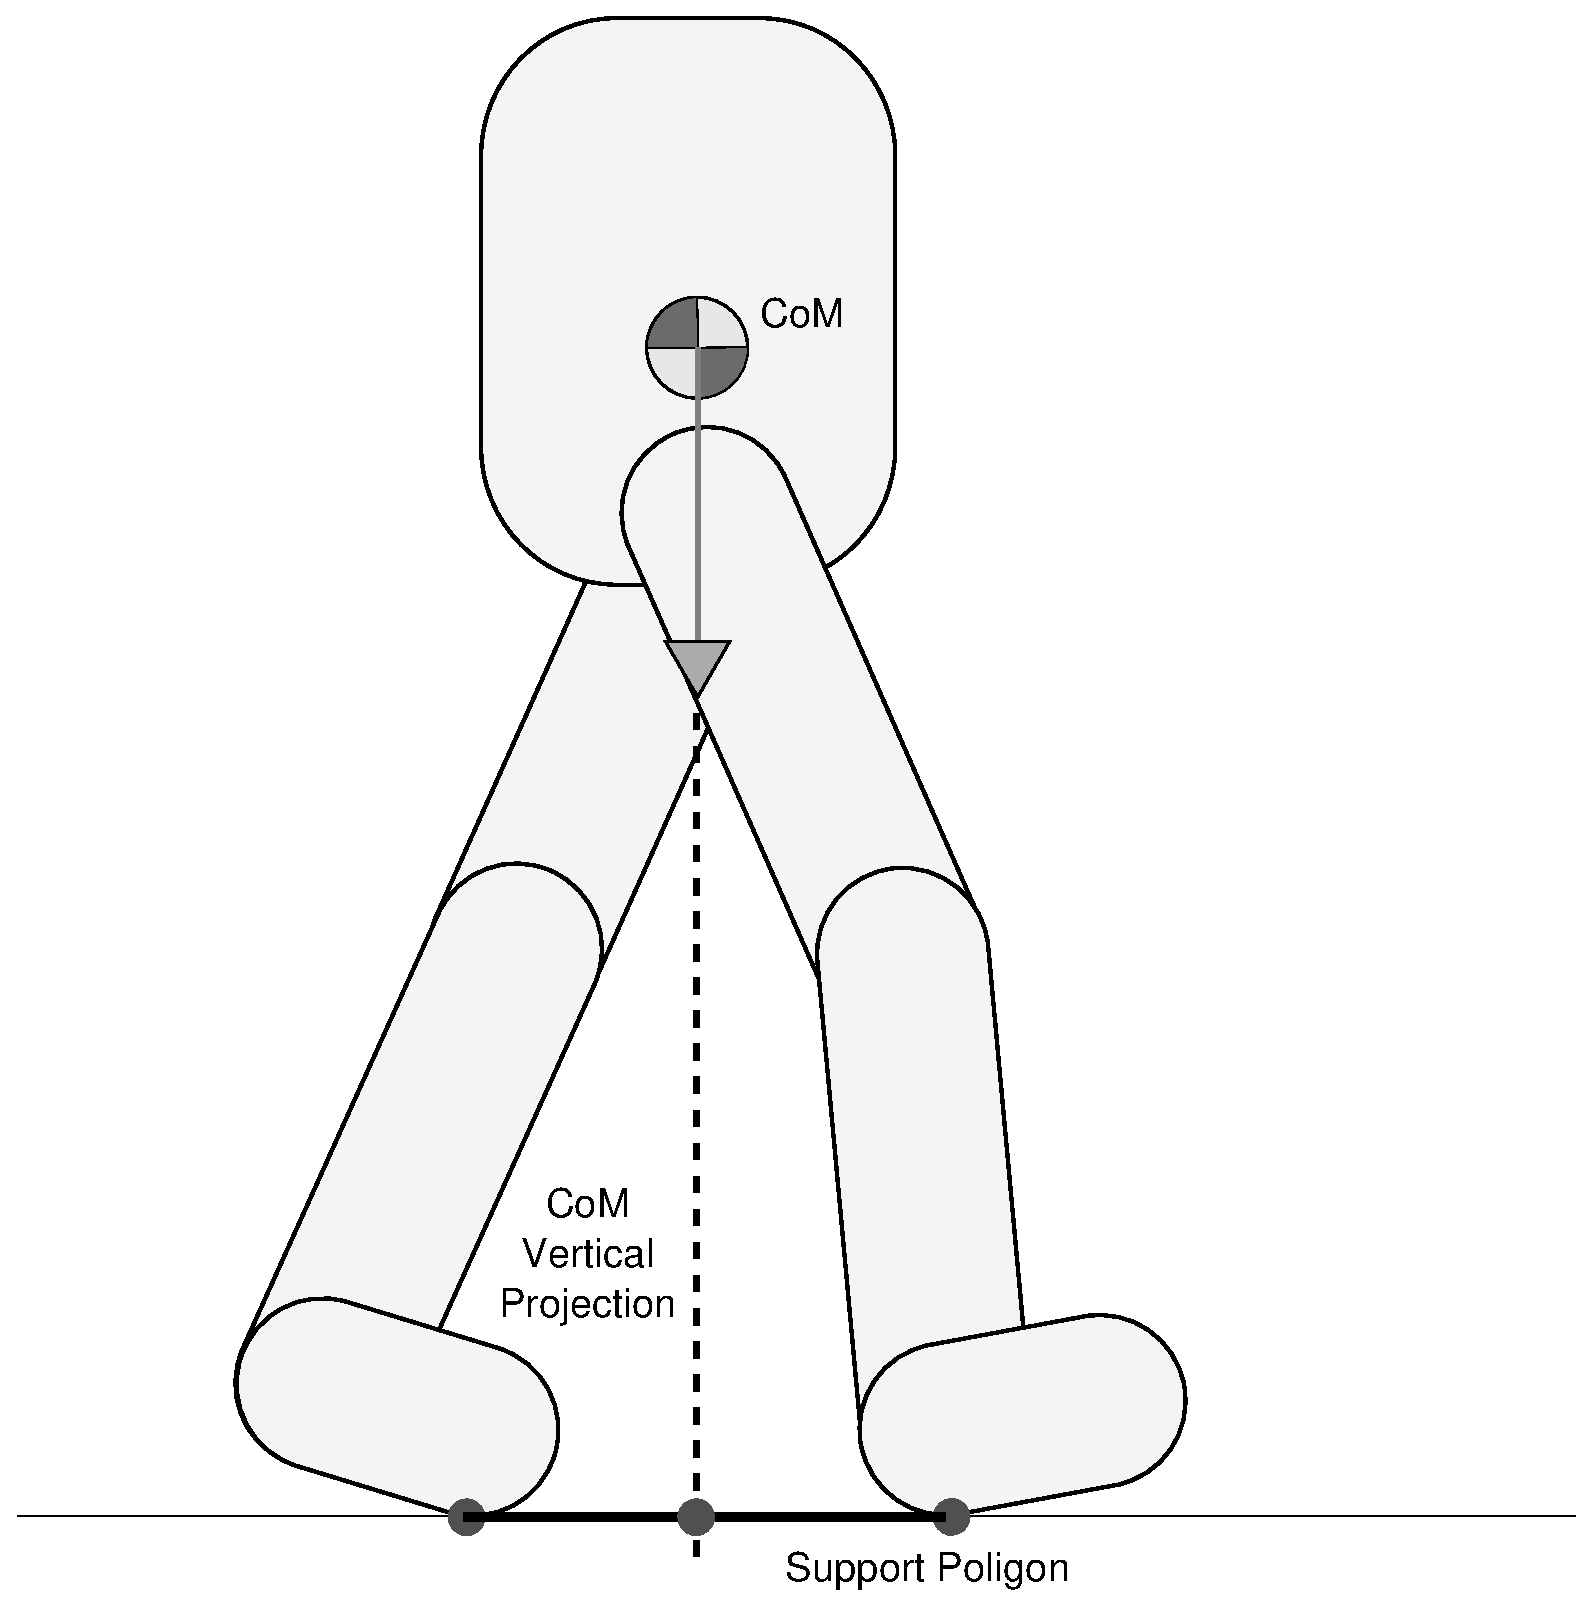
\includegraphics[scale=0.3]{FigRobotCoM}
%   \end{center}
%   \caption{Static Equilibrium by CoM vertical projection over
%     support polygon.}
%   \label{fig:FigRobotCoM}
% \end{figure}

The second method, takes in account the inertial forces due to
dynamical motion, and its general definition is still and open problem
\cite{Azevedo04Artificial}. However, a limited way to determine biped
dynamic equilibrium is given by the projection of the dynamical
equivalent to CoM: the Zero Moment Point (ZMP). The Zero Moment Point
is the point where the reaction force with the supporting element
would produce a zero moment. If the ZMP is located inside the
supporting polygon, unstabilizing moments due to dynamic locomotion
would be compensated by the support reaction. An illustration of a
robot which is not in equilibrium is shown in
Fig. \ref{fig:FigRobotZMP}. The ZMP is the projection over the floor
of the total force acting over the CoM. When accelerations become
relevant, the reference frame placed in the CoM is not anymore an
inertial frame and, therefore, appears an inertial force opposed to
CoM acceleration, which, with the weight force, yield a total force
not normal to the floor. In order to be in moment equilibrium, the
projection over the floor of the total force must coincide with the
floor reaction point, that is, the point where the equivalent reaction
force is applied.


% \begin{figure}
%   \begin{center}
%     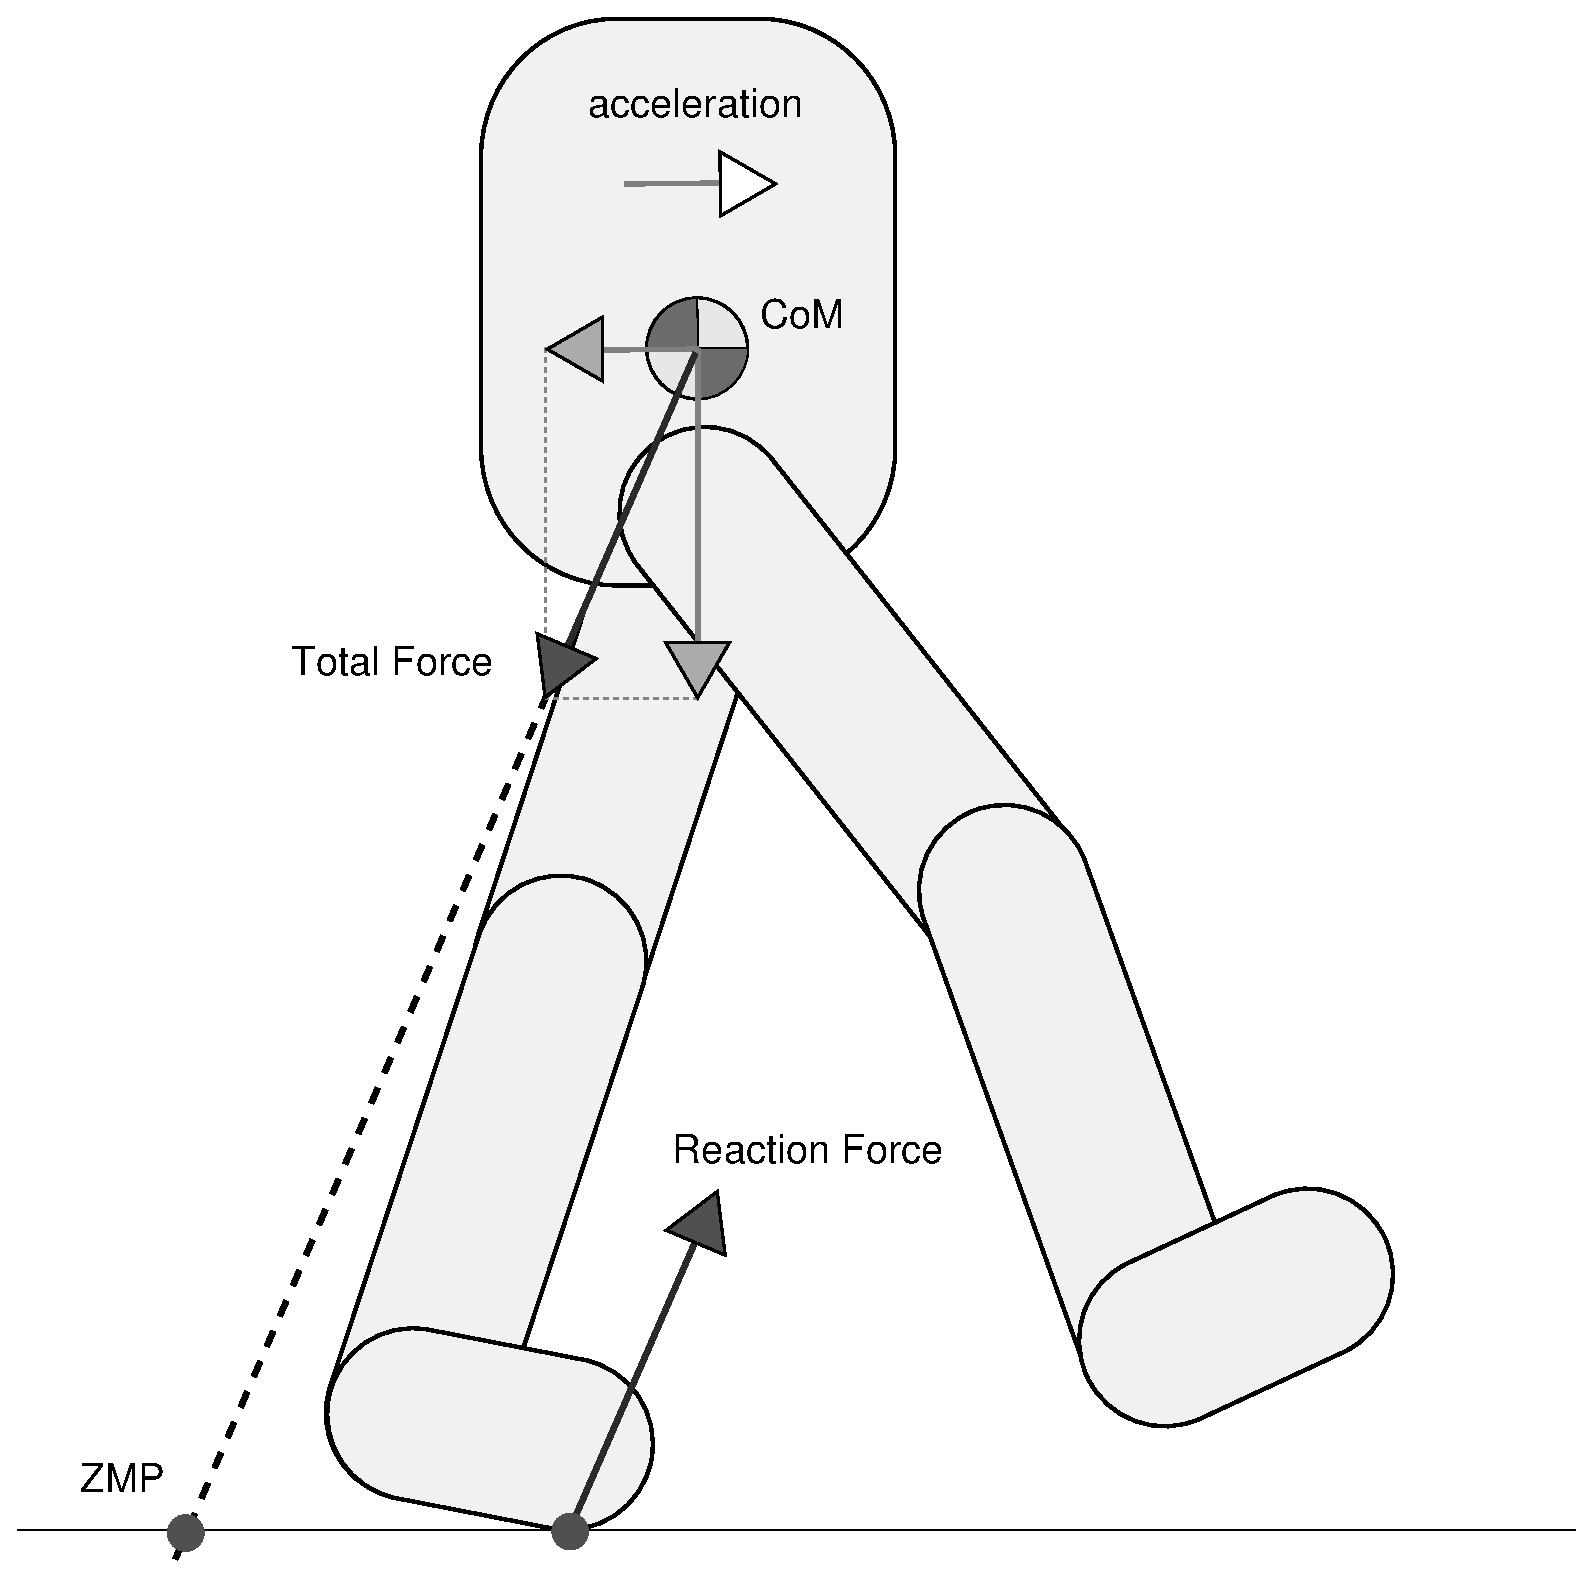
\includegraphics[scale=0.3]{FigRobotZmp}
%   \end{center}
%   \caption{Dynamic Equilibrium not attained because of ZMP and floor
%     reaction point not coincident. The robot is falling backwards.}
%   \label{fig:FigRobotZMP}
% \end{figure}

Biped locomotion can be thought as a rhythmic and symmetric
progression of trunk and limbs movement. In a complete gait cycle each
leg passes trough a stance phase, in which its toe is in floor
contact, and a swing phase, in which the foot is balancing without
floor contact. Between them is a double support phase, where both feet
are conforming the support area. Double support phase dynamics is more
complex than that of the single support because of the additional
constraints that yields a parallel kinematic chain. Thereby, a usual
modeling technique is to model the dynamics of single support and a
punctual transition condition for the double support
\cite{Garcia98simplest}. However, double support dynamics modeling
could be representative since it accounts for 20\% of the gait cycle.


\subsection{Biological Considerations on Biped Locomotion}


In order to build suitable controllers for biped locomotion it is
necessary to define what aspects, or features, are most important to
good performance, robustness, stability, adaptability, and optimality
of walking. All of these properties are attained by biological biped
walking and therefore it is the main inspiration for building models
as well as controllers of locomotion.


There are several models of biped walking, and each of them remarks
one or more important features. A very good review and analysis of
biped locomotion models can be found in
\cite{Vaughan03Theories}. Vaughan reviews six models of bipedal
walking: Bipedal walking as an evolutionary adaptation of hominids,
minimization of energy consumption by displacing the CoM along an
optimal path, progressive learning with risk of falling minimization,
spinal cord interneurons acting as rhythmic central pattern
generators, neural system training along with biomechanical system and
environment adaptation, and feedback control in powered dynamic
locomotion. The neurobiological aspects of motion control have been
examined in \cite{Duysens02walking}. Duysens remarks the reflex
response of sensor inputs in motion control and presents tree levels
for neural motion control: Feedback control in motoneurons, in terms
of contribution of reflex action over motoneuron signal intensity;
feedback control in central pattern generator flexor-extensor centers,
relevant to movement synchronization and reflex response to
perturbation and loads; and higher level control, referred to
conscious control of locomotion. Duysens states that despite of the
relative low understanding of the high level control participation in
locomotion, the two lower levels are complex and rich enough to be
studied an applied to robot design (i.e. the so-called {\it spinal
  robot}, because it would have the control architecture expected in a
human with transected spinal cord).



% \subsection{Robustness and Non-structured environments}


% \subsection{Planning Beyond Periodic Walking}


\section{Neural Fields}
Neural fields arise as a tissue level model of neural populations in
brain. It has been proposed by Wilson and Cowan
\cite{Wilson72Excitatory} and detailed by Amari \cite{Amari77Dynamics}
in the particular case of lateral inhibition. In this model, neural
population in considered continuum in which exists a dynamical
evolution equation where the mean activation potential evaluated in
one place is affected by its neighborhood according to a so-called
mexican hat function (as noted by Coombes \cite{Coombes05Waves} better
called wizard hat function) in which close neighbors act as exciters
and distant ones act as inhibitors.

The base model, as presented by Amari \cite{Amari77Dynamics} for the
multiple layer case is:

\begin{equation}
  \label{eq:nf-base}
  \tau_i\frac{\delta u_i(x,t)}{\delta
    t}=-u_i+\sum_{j=1}^{m}{\int{w_{i,j}(x,x';t-t')f_j\left(
        u_j(x',t')\right) dx' dt'}+h_i+s_i(x,t)}
\end{equation}

Where $\tau$ is a temporal constant of synaptic decay rate, $u_i(x,t)$
is the average membrane potential of the neurons located at position
$x$ at time $t$ on layer $i$ (where $x$ can be 1-dimensional,
2-dimensional or even of higher dimension). The average intensity of
connection from neurons on layer $j$ at $y$ to neurons on layer $i$ at
$x$ is modeled with $w_{i,j}(x,y)$, $f_j(\cdot)$ is the saturating
output function which is monotonically nondecreasing. The deviation of
the average stimulation potential at place $x$ at time $y$ of layer
$i$ is represented by $s_i(x,t)$, and $h_i=\bar{s_i}-r_i$ is the sum
of the average stimulation potential an the resting potential of layer
$i$.


There are several assumptions that produce simplifications over the
previous model. One of them is to include the additional dependence of
the time lag of signals $t'=\lvert x-x'\rvert /v$ where $v$ is the
velocity of an action potential
\cite{Wilson72Excitatory}. Nonetheless, while not stated otherwise we
will not take into account the time lag, as well as the multiple
layers. We will also merge the non-homogeneous terms
$S(x,t)=h+s(x,t)$. This way, the resulting equation takes the form
(for $x$ $n$-dimensional):

\begin{equation}
  \label{eq:nf-simp}
  \tau \frac{\delta u(x,t)}{\delta
    t}=-u+\int_{\mathbb{R}^{n}}{w(x,x')f\left(
      u(x')\right) dx'}+S(x,t)
\end{equation}

For further simplification, temporarily we will consider the
connection kernel $w(x,x')$ as isotropic and homogeneous, so that it
only depends on the norm of the vector difference $\lVert x-x'\rVert$
i.e. $w\left( \lVert x-x'\rVert \right)$. Amari found diverse
stable-state solutions for the one-dimensional case (isotropic and
homogeneous), where the model is:

\begin{equation}
  \label{eq:nf-oned}
  \tau \frac{\delta u(x,t)} {\delta
    t}=-u+\int_{-\infty}^{\infty} {w\left( \lvert x-x'\rvert \right)
    f\left( u(x') \right) dx'}+S(x,t)
\end{equation}

The typical form for the connection kernel (for which Amari obtained
his results) can be seen in figure \ref{fig:wiz-hat}.

\begin{figure}[h]
  \centering
  \caption{Wizard hat function used as connection kernel.}
  \label{fig:wiz-hat}
\end{figure}

Also, the typical sigmoid saturation function, as well as its maximum
gain limit case (the Heaviside function), are shown in the figure
\ref{fig:sat-fun}.

\begin{figure}[h]
  \centering
  \caption{Sigmoid and Heaviside saturation functions.}
  \label{fig:sat-fun}
\end{figure}


% \section{Neural Fields}

% \subsection{Mathematical Model}
% \subsection{Local Solutions}
% \subsection{Bifurcation and Modes}


\section{Evolution and Adaptation}
\subsection{Evolutionary Algorithms}
Evolutionary algorithms are a set of population-based heuristic search
and optimization techniques. They maintain a population, and apply a
set of operators or transformations over its members. Those operators
are typically inspired on biological evolution and usually include
selection, reproduction and mutation, among others. The operators are
dependent of the evaluation of a performance function called fitness
function. Generally, fitness function evaluation may include, from a
simple numerical evaluation, to a complex simulation, in order to get
the performance criterion which its optimization is pursued.

The pseudo-code of a general evolutionary algorithm is as follows:

\algsetup{indent=2em}
\begin{algorithm}[h!]
  \caption{$Evolutionary Algorithm$}\label{alg:factorial}
  \begin{algorithmic}[1]
    \STATE $P \leftarrow$ Generate initial population of size $N$
    \STATE Evaluate fitness for each individual in $P$ \REPEAT \STATE
    $P' \leftarrow$ Apply operators to $P$ \STATE Evaluate fitness for
    each individual in $P'$ \STATE $P \leftarrow$ Select $N$
    individuals in $P'$ according to a selection scheme
    \UNTIL{Termination condition is met}
  \end{algorithmic}
\end{algorithm}

The most predominant form of an evolutionary algorithm is embodied by
genetic algorithms. They most frequent genotypical representation is a
bit sequence, although other representations can be used. Usually they
are implemented with a generational replacement of population, but in
some situations it is useful to conserve a small set of the better
individuals across generations in a steady-steady replacement.

% \subsection{Niching}
% \subsection{Dynamic Environments and Co-evolution}


\section{Computational Intelligence Applied to Biped Robotics: A
  Survey}
% \begin{figure}
%   \begin{center}
%     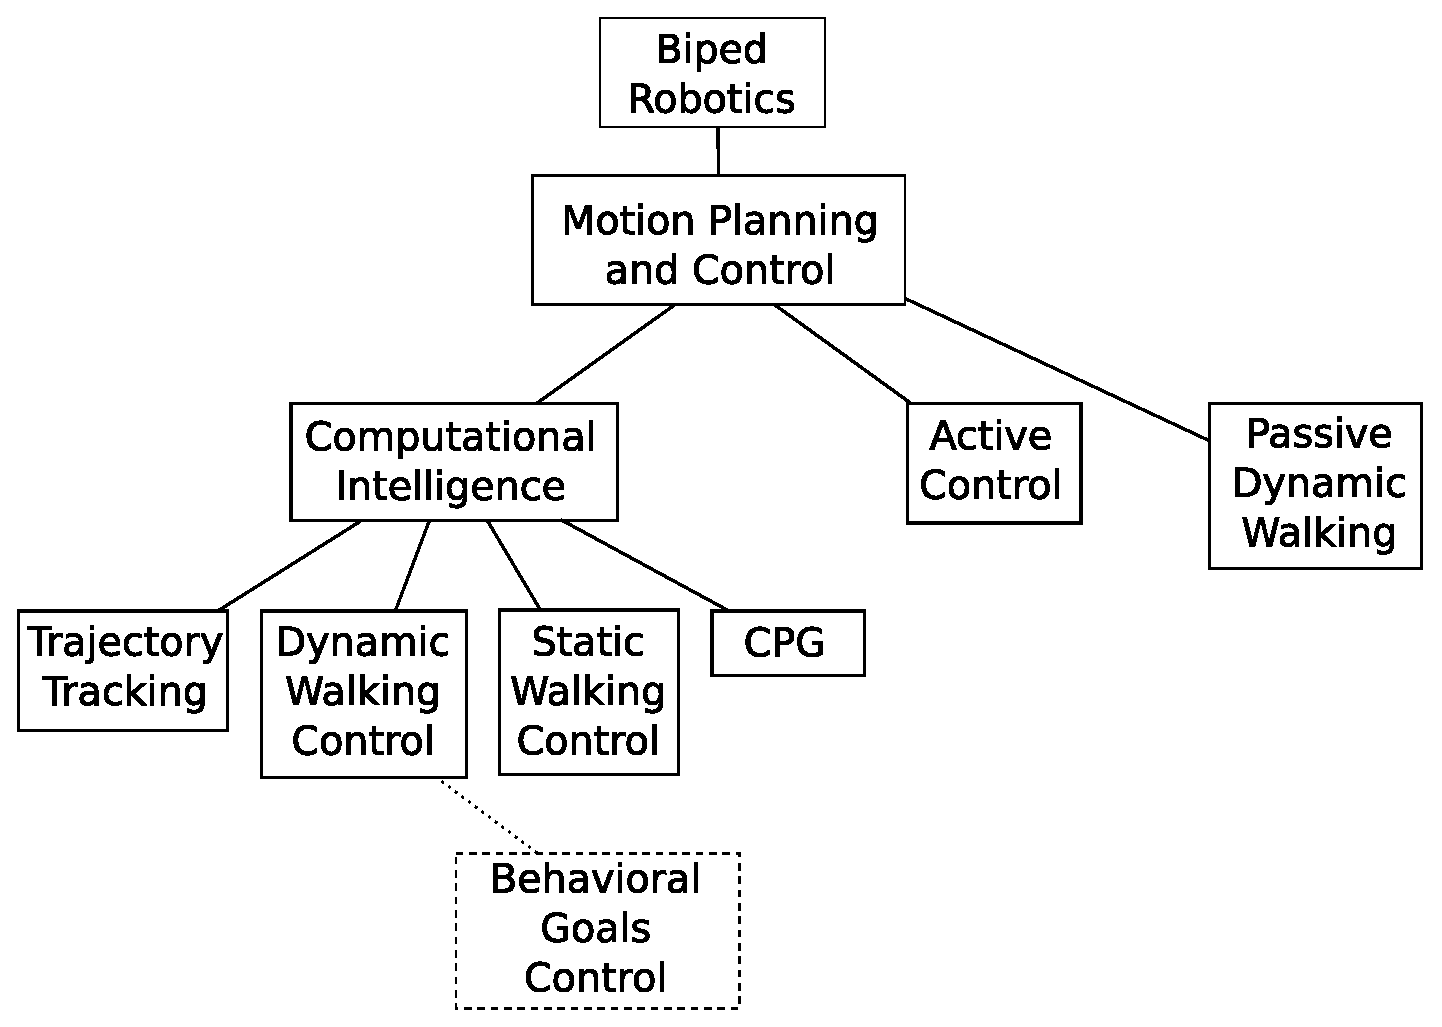
\includegraphics[scale=0.7]{FigTaxonomyTree}
%   \end{center}
%   \caption{A taxonomy tree of motion planning and control methods in
%     biped walking}
%   \label{fig:FigTaxonomyTree}
% \end{figure}

Here is presented a tentative taxonomy of the previous works made in
the area of motion planning and control methods in biped
walking. Three major approaches are identified: Computational
Intelligence, Active Control and Passive Dynamic
Walking. Fig. \ref{fig:FigTaxonomyTree} shows for a graphical
representation of the taxonomy with emphasis in computational
intelligence methods.


Before focusing on computational intelligence methods, the two other
methods mentioned are briefly presented.


Active Control refers to the persistent control of the joint actuation
and state applying control theory. It includes position, velocity,
acceleration and torque control techniques. Also, several design
methods can be used, including some derived from linear ones but
applied to nonlinear systems. In the methods used are included methods
based on frequency response, performing the optimization of a
performance criterion (e. g. H$_\infty$ control), or applying state
feedback. Another simpler method used is the tuning of parameters of a
PID controller. Also it is possible to a given extent use local linear
approximations and directly use linear control methods. Active control
gives the best trajectory tracking and accuracy, provides methods to
evaluate stability (such as Lyapunov stability analysis), and can be
vertically integrated to higher motion planning algorithms, but its
main deficiency is its very high energy consumption due to the
persistent control of joint actuation, even when optimal control is
applied.

The other major approach is Passive Dynamic Walking (PDW). In PDW it
is took the opposite approach by totally suppressing any joint
actuation. The idea is that the actuation given by gravity force over
a biped robot standing over a slightly inclined surface, in
conjunction with its natural dynamics, must achieve stable gait
patterns. This is attained by using passive elements as springs and
dampers and a careful mechanical design guided by a detailed analysis
by dynamic systems theory, including state space modeling, phase
transitions, and probably other techniques such as Poincarè maps and
Lyapunov stability analysis and, mostly, dynamic simulation. In order
to obtain gait pattern in flat surfaces it can be applied
reinforcement learning in a control system so as to learn how to
simulate the slight actuation given by the gravity in the inclined
surface case. The main advantage of this method is its very low energy
consumption, and its main disadvantage is its low flexibility to track
general paths, particularly those including vertical movements, and
its high sensibility to environment conditions.

Next, each one of the three major approaches to the problem that apply
computational intelligence are examined. These are Central Pattern
Generator methods, Dynamic Walking Control methods, Static Walking
Control methods, and Trajectory Tracking methods. This classification
emphasizes the way in which the problem is solved and not the subfield
of computational intelligence used.

\subsection{Central Pattern Generator (CPG) Methods}
A Central Pattern Generator (CPG) is a system which is supposed to
give the coordinated rhythmic stimulation to joints required to
generate a gait pattern. It is inspired from the spinal motor center
find in animals such as mammals, and it is usually implemented using a
kind of neural networks called oscillatory neural networks.


Neural oscillators are a special type of artificial neural networks
(ANNs) described by two essential elements: the dynamical properties
of the individual neuron, and the type of coupling between
neurons. Each neuron has its dynamics described by a set of
differential equations.


% \begin{figure}
%   \begin{center}
%     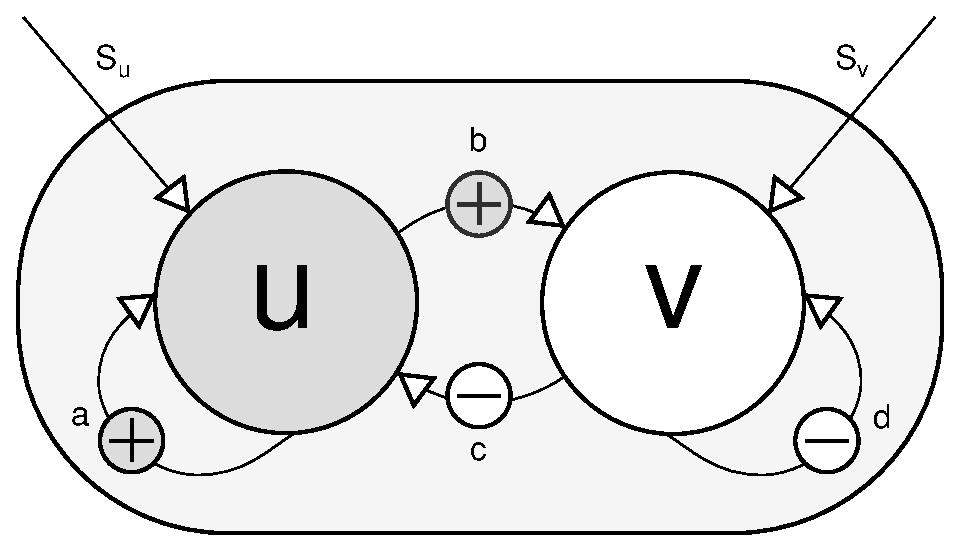
\includegraphics[scale=0.4]{FigNeuralOscillator}
%   \end{center}
%   \caption{Topology of an Amari-Hopfield neural oscillator}
%   \label{fig:FigNeuralOscillator}
% \end{figure}

A more specific model of neural oscillators couples neurons in
pairs. It is based in the fact that most muscle fibers have one
excitatory center for flexion and another for extension, and them are
inhibiting between them. This way, the two coupled neurons can be
represented by a set of differential equations. An example of this
arrangement is the Amari-Hopfield model, for which a grafical
representation is shown in Fig. presented here as shown in
\cite{Nakada2003}:
\begin{eqnarray}
  \tau\dot{u}=-u+af(u)-cf(v)+S_u(t) \\
  \tau\dot{v}=-v+bf(u)-df(v)+S_v(t)
\end{eqnarray}
In which $u$ and $v$ are the neuron potentials, $S_u(t)$ and $S_v(t)$
are the respective neuron inputs as function of time, and $f(u)$ and
$f(v)$ are neuron outputs after applying the transfer function:
\begin{equation}
  f(x)=\frac{1+tanh(\mu x)}{2}
\end{equation}


The parameters $a$, $b$, $c$ and $d$ characterize the neural
oscillator behavior. This kind of arrangement is typically followed in
the CPG control methods, where each neural oscillator (neuron pair) is
used to stimulate a single joint, and the mutual interaction of neural
oscillators conform the CPG.


A classical author in the application of CPGs to motion control of
biped locomotion following the methodology presented above is Taga,
who in his preliminary work of 1991 (see \cite{Taga1991}) applied the
concept of coupled neural oscillators, remarking the self-organizing
properties of the neural system with the physical system and the
environment, which gives some disturbance rejection that keeps the
equilibrium of biped walking.
 

In general terms, the neural oscillator can be thought not only as the
coupling of two neurons, but more globally, the rate of neuron
activation potential variation can be a function of the network
inputs, its current activation potential and a special term called
fatigue. Also the rate of variation of fatigue is function of the
current fatigue and its current output. A general expression for the
system of differential equations that rule the dynamics of a
individual neuron is \cite{Cao98design}:

\begin{eqnarray}
  \tau_r\dot{x_i}=-x_i+\displaystyle\sum_{j=1,j\neq i}^n a_{ij}y_j-bf_i+s_i \\
  \tau_a\dot{f_i}=-f_i+y_i \\
  y_i=H_1(x_i)x_i \\
  H_1(x)=\displaystyle\left\{ \begin{array}{cc}
      1 & x\geq 0, \\
      0 & x < 0, 
    \end{array} \right.
\end{eqnarray}


Here, $x_i$ denotes the activation potential of the $i$th neuron,
$y_i$ its output, $a_{ij}$ the connection weight from neuron $j$ to
neuron $i$, $f_i$ is the fatigue strength, $b$ is the coefficient of
fatigue, $s_i$ is a bias factor, and $\tau_r$ and $\tau_a$ are time
constants.


With this model Cao and Kawamura used an oscillatory neural network as
CPG to generate biped walking patterns. The net composition includes a
single neuron for each articulation, and all neuron are connected
between them (i. e. all the networks is a single coupled neural
oscillator). The neuron activation function is given by the set of
equations presented above. A connectivity matrix, with inhibitory and
excitatory weights (composed by the different terms $a_{ij}$) was
evolved using an genetic algorithm to obtain a gait pattern. The
chromosome is a linear arrange of matrix elements in binary
representation in the form:


\begin{center}
  $\begin{array}{cccccc}
    < & \underbrace{b_0b_1\dots b_7} & \underbrace{b_8\dots b_{15}} & \dots\dots & \underbrace{b_{440}\dots b_{447}} & > \\
    & a_{12} & a_{13} & & a_{87} &
  \end{array}$
\end{center}


The fitness function used is dived in two partial qualitative
functions and a third which evaluates the correctness of the gait,
applying three genetic algorithms, one nested in another (authors
called it hierarchical evolutionary algorithm). This way they were
able to control eight joints and generate successful gait patterns.
 

Next is presented relevant previous works that mainly use Central
Pattern Generators as motion strategy.

Kun and Miller \cite{Kun96Adaptive} implemented a control for biped
robot walking of a 10-DOF robot, for which they used a CPG that uses a
heuristic to generate sequences, synchronizing the performance in the
joints with the natural dynamics of the robot, and receiving
correction parameters in the lateral and frontal motion given by CMAC
neural networks as inputs. Additionally, a third CMAC network is
trained to help control the robot in the double support phase. The
natural dynamics of the robot is fundamental for the control system
given its dependency on directional balance to stabilize the
movement. They used temporary difference learning to train
networks. This pioneer work is validated implementing it on a real
biped robot.


Venkataraman \cite{Venkataraman97simple} made a complete compilation
of the important elements in the CPGs in the field of biology and the
robotics, and proposes an alternative method for biped, quadruped and
hexapod locomotion patterns generation. The method has relation with
the general implementation using oscillatory neural networks, but
unlike these, it employs a single linear patterns generator, with
which the movements are generated in each extremity using filters of
finite dimension (adjustments of phase lead and phase lag filters) to
simulate the delays that produce the coordinated movement necessary
for locomotion. The oscillator is modeled including elements of the
Van der Pool oscillator to obtain a nonlinear system with a robust and
stable focus. There are presented as result patterns for the gait
types already mentioned, proving that they can be obtained with a
simple architecture.


Benbrahim and Franklin \cite{Benbrahim97Biped} developed a CPG using
CMAC neural networks and simultaneously applying reinforcement and
supervised learning. They use a central network, the generator, aided
by a set of peripheral control networks in parallel with observation
networks, whose inputs are relevant parameters that act as gait
restrictions, among them body posture and height of body mass
center. Peripheral control networks act only if its correspondent
observation network detects a improper behavior from central network
for a specific restriction. Control system output is determined by a
Gaussian function with median located in the CPG output and standard
deviation that initially has a high level and reduces as solution
converges. Dynamic control necessary to follow the reference provided
by CPG is easily implemented with a set of PID controllers. In the
real application, the control scheme was aided by a posture bang-bang
control (i. e. on-off control). It was required a previous training in
order to obtain suitable network training time. This novel approach
allows to prevent that CPG errors cause a general gait failure, not
only providing robustness but accelerating the learning process.


Hasegawa et al. \cite{Hasegawa00Trajectory} proposed a method for
developing pattern generators useful for a biped 13-DOF robot walking
on inclined surfaces. They solved the unconstrained optimization
problem with a hybrid evolutionary algorithm with a lower layer that
generates trajectory points (from a cubic spline) using evolutionary
programming (EP), which are added in interpolated point sets, and
those set are in time evolved using a genetic algorithm (GA),
selecting the successful sets that minimize energy consumed by the
robot. Due to that each point evaluation depends on the best
individual in the GA layer, and also second layer individuals a sets
of elements of the first layer, the algorithm has a co-evolutionary
scheme. In the practical implementation made, the dynamic control is
performed by PD controllers.


Reil and Husbands \cite{Reil02Evolution} used an evolutionary
algorithm (EA) to optimize the parameters of a fully connected
recurrent neural network. The model of each neuron is a dynamic model
that attenuates its answer in stimulation absence, and depends on a
set of weights, a bias factor and a dynamic time constant, with a
dynamics similar to the model exposed previously and presented in
\cite{Cao98design}. The three parameters types for the totality of
network neurons are represented linearly in the individuals genotype
used in the evolutionary algorithm. The fitness function used favors
movement that maximizes displacement in frontal direction and
penalizes movement in vertical direction. The authors manage with such
simple evaluation rule to generate satisfactory patterns of march
without any sensory feedback. Later, they add a sensorial entrance of
auditive type and, leaving the recurrent connections fixed, they
evolve the recurrent neurons connection weights with the sensory
input. This way, they attain that the robot navigate towards a source
of sound emission. The neural controller generates reference points
that are taken to forces in the motors by a PD torque control. An
addition to the efficiency of the algorithm is the premature
abandonment of marches that move strongly in vertical direction. They
have achieved a relative low success rate in evolutions (close to
20\%) and propose switching to a more traditional CPG method.


Miyashita et al. \cite{Miyashita03Evolutionary} recalled the
conceptualization of previous authors like Taga, emphasizing the
importance of the oscillating behavior in the nervous system in form
of CPGs. The proposed controller this way is based on oscillating
artificial neurons, or oscillators, which are connected mutually in
pairs to obtain a periodic behavior, in a form similar to the
Amari-Hopfield model presented previously. It is shown the evolution
of neural network structure using genetic programming (GP), in terms
of the interconnections between oscillators, supposing the internal
structure of the oscillators fixed (i.e. the parameters $a$, $b$, $c$,
$d$ an $\tau$). The GP implementation for solving the problem is made
representing the local network from each oscillator like an
S-expression, doing a co-evolution where a subpopulation for each
oscillator is evolved, but the evaluation of the aptitude function as
well as the application of genetic operators are applied over an
oscillator group, each one of a different population. Results of walks
generated with this method are displayed, until a maximum of 10 stable
steps. This work, spite its relative success, has a very large
computational overhead and gives a very small set of successful neural
oscillators. Nonetheless, its approach is very illustrative, and
somehow resembles the spinal control proposed in
\cite{Duysens02walking}.


Paul \cite{Paul03Bilateral} argued that, unlike the controllers that
use a CPG whose connections between oscillators in left and right
sides are connected, it is possible to obtain a satisfactory biped
walking with two decoupled generators. Two cases area treated: the
first one decouples control and sensor system, having each an
independent CPG, without any connection to each other and with
entrances of sensors strictly located in his partial side; while the
second one decouples connections but allows common entrances to both
global position sensors. Both controllers are evolved in parallel with
genetic algorithms (GA) to three morphologic parameters. It is shown
that for the first case successful biped walking is achieved in most
of cases but there are problems to follow a straight line. In the
second, it is shown that the CPGs decoupling with global entrances is
an equally satisfactory technique that the entirely coupled case. This
way, Paul gives a highly valuable approach, in which a lot simpler
technique achieves similar results to those more complex traditionally
used. Paul therefore hypothesizes that lower limb control in walking
is inherently reactive and sensory-motor coordination based, and CPGs
are used only to alter gait conditions acting only in the trunk and
arms.


In the another work \cite{Paul04Sensorimotor}, Paul aimed to continue
the work oriented to controller simplification for the biped walking
based on neural networks, this time showing that independent simple
networks for controlling each leg can generate a stable walk, using
only forward connections (i. e. a feed-forward neural network) without
hidden layer. The used networks only receive as entrance the contact
with their respective leg and a common bias signal for both
controller. Of numerous configurations evolved with genetic
algorithms, only two obtained the satisfactory long walk, but in a
remarkable form, both indefinitely turned out to be stable. It is
used, like in previous works of Paul, coevolution of some few
morphologic parameters. This is probably the simpler solution to this
problem proposed to the time.


Nakanishi et al. \cite{Nakanishi2004b} made a less traditional
approach to the generation of patterns for biped walking with some
similarities to the CPGs. The idea consists of designing oscillators
represented as systems of nonlinear phase coupled differential
equations, in such form that the fundamental element of dynamics is
not the oscillation frequency of each element, but its phase relations
in order to obtain a desired movement pattern. A local weighted
regression (LWR) is proposed as a training scheme to adapt elements
phase, as well as dynamic system global oscillation
frequency. Additionally, it is applied the concept of phase reset at
the moment of heel strike. It is shown that the phase reset principle
is advantageous when disturbances in real robot walking appear. Also,
it is argued that the phase controller is simpler to train than
CPGs. They also affirm the presented controller superiority in front
of a controller by finite automata. It is remarkable that this work,
first, abstracts the concept behind CPGs and, second, employs the
already biologically supported phase reset. A minor flaw of this
method is its high sensibility to initial conditions.


Komatsu and Usul \cite{Komatsu05Dynamic} showed the control for
different biped locomotion types using Hybrid Central Pattern
Generators (H-CPG). The total action of the H-CPG proposed is
determined by the sum of the individual actions of each one of its
components: A neural oscillator that generates the rhythmical patterns
in form of torques, a support force controller that applies the
Jacobian matrix to map forces from cartesian space to joint space, and
a position controller that implements a PD control to maintain legs as
vertically as possible. The vertical and horizontal movements are
separately processed by the force controller. They shown that proposed
method allows to vary form slow walking to rapid walking, and also
walking and running in modified environments, particularly in
slopes. Satisfactory results were obtained in simulations and real
robot implementation, and a high movement versatility was attained by
complementing traditional CPG techniques with force and posture
control. The system complexity in not so high and is indeed feasible.

Computational intelligence methods used are:
\begin{itemize}
\item Oscillatory Neural Networks: As nuclear elements of CPGs.
\item Evolutionary Optimization: For optimization and training of CPGs
\item Rhythmical Dynamic Systems: An alternative to oscillatory neural
  networks for building CPGs.
\end{itemize}
\subsection{Trajectory Tracking Methods}
Methods included in this category largely vary in implementation, but
its main methodology consists of generating a kinematic pattern or
succession, in a way that the joint following of it yields a
successful gait pattern. Although there are applied computational
intelligence methods in generating the trajectory, this process is
typically followed by a simple control method, such as a PID
control. Developments under this approach are relatively recent and
have strong foundation on evolutionary computation methods.


The work of Capi et al. \cite{Capi02Optimal} gave and approach to
obtaining a stable biped walk with an optimal power consumption for a
biped robot of prismatic joints. The control system is based on the
principle of Zero Moment Point (ZMP). The control loop for center of
gravity (of PD type) receives a reference of the center of gravity
location of the robot, and generates a control signal that receives
the ZMP control loop, along with the current ZMP location. In the same
way, the ZMP control loop processes that information and outputs
actuation values for the rotational joint in the feet and the
prismatic joint in the thigh. A genetic algorithm with real
codification is used (equivalent to an evolutionary strategy) to look
for the reference trajectory that generates the minimum energy
consumption. The results with the optimization for minimum torque
applied and optimization for constant height of center of gravity are
compared. The problem of optimization with restrictions is turned to a
problem without restrictions to which penalties in the aptitude
function are added when the conditions of restriction are failed to
fulfill. This way, Capi et. al present a gait trajectory generation
method for an unusual robot configuration, and also give a forward
step to optimization of energy consumption using evolutionary
computation.


Later, Yamasaki et al. \cite{Yamasaki03Control} applied the evolution
by genetic algorithms (GA) to design a controller for a biped walker
with low torque consumption. For it they proposed the optimization of
the gait sequences generated in two phases. The gait sequences in
terms of speeds are described like a set of sinusoidal functions with
amplitude and phases as parameters, dependent on the angular positions
of both legs. The parameters described are optimized along with the
functions global angular speed. A binary representation is used,
applying cross and mutation operators. The algorithm is divided in two
phases, first with a fitness function proportional to total distance
walked by the robot during the simulation time (or before falling),
and the second one proportional to the walked distance and inversely
proportional to the used energy. Therefore, a sequential optimization
is made in order to, first, obtain suitable gait trajectories, and
second, minimize energy consumed. Nevertheless, the best trajectory
obtained attained less than 2 second of walking before falling, and
this should be regarded only as a partial success.


Garder and Howin \cite{Garder06Robot} recently applied a hybrid method
of genetic algorithms (GA) and hill climbing to evolve walking
patterns for a biped robot with pneumatic actuation. In the problem
faced by them, the movement of the robot is restricted to sagittal
plane, as to it is of concern only the robot frontal advance. The
genotypical codification used is binary, and the complete sequence is
represented by an individual, divided in three mechanism positions
with pause times between them. The chosen method consists of leaving
the durations fixed and using a traditional genetic algorithm to
evolve the three positions that characterize the sequence of movement
by 8 generations, and later to make an optimization by hill climbing,
leaving fixed the bits of position, and generation after generation
optimizing from the most significant bits of pause times to less
significant ones. Satisfactory locomotion in the form of synchronous
jumps is obtained. The short run time of the algorithm allows to
implement it in real time in the robot. The result obtained where
facilitated by the low problem dimensionality and relative smoothness
of fitness landscape, but the method can fail on more complex
problems.


Contemporarily Yanase and Iba \cite{Yanase06Evolutionary} presented an
implementation of an evolutionary algorithm with user interaction to
determine sequences of movement, as well as other implementations with
specific functions of aptitude to reach certain objectives. In the
first case, the optimization of a sequence of movement by interactive
evolutionary computation appears (IEC), for which a set of
alternatives for each picture of movement is generated (keyframes),
being these evaluated by the user graphically and, applying
evolutionary operators in successive iterations along with the
evaluation mechanism, each one of the pictures that are to form the
sequence is obtained. Later they show how specially designed fitness
functions can be used, altogether with a dynamic simulator, to
optimize the movement to seat or kicking a ball. Also, they make a
brief reference to the implementation of an multiobjective genetic
algorithm (MOGA) for the solution of such problems. This is a novel
approach in the fitness dynamical user evaluation employed and also in
the alternative objective based approach to evolution.

The application of computational intelligence methods in this approach
is focused on:
\begin{itemize}
\item Evolutionary Computation: For optimization of trajectories under
  a performance criterion (such as energy consumption, stability or
  specific motion objectives).
\end{itemize}

\subsection{Dynamic Walking Control}
These are probably the most complex methods among those based on
computational intelligence. They aim to obtain dynamic stable walking
by a control based on various techniques. Among them are included
neural networks, fuzzy systems and evolutionary algorithms.


Some concepts used in this section have been already presented, but it
is useful to detail recurrent neural networks, which are an important
and promising technique. A recurrent neural network is usually modeled
as a fully connected network without layered structure
\cite{Haykin98Neural}, in which the output can be expressed in
vectorial notation as a linear combination of neuron states:

\begin{equation}
  y_{rnn}(n)=C x_{rnn}
\end{equation}
\newline And neuron states in $n+1$ are a function of recurrent
potentials and input potentials in $n$, each of them multiplied by
weight matrices.

\begin{equation}
  x_{rnn}(n+1)=\varphi(W_a x_{rnn}(n)+W_b u_{rnn}(n))
\end{equation}
\newline The function $\varphi()$ is a diagonal activation function,
usually of sigmoidal shape. This way, a recurrent neural network is a
dynamical system determined by its weight matrices $W_a$ and $W_a$,
its activation function $\varphi()$, and the linear combination of
states used as output $C$. The relevant capability so obtained is that
recurrent neural networks not only are a nonlinear mapping from inputs
into outputs, but they present memory and dynamical response to
inputs, which can give birth to emergent behaviors.


Next, some works in the field of dynamically stable walking are
presented, beginning with the preliminary work of Magdalena and
Monasterio-Huelin using fuzzy systems.


The work of Magdalena and Monasterio-Huelin \cite{Magdalena97fuzzy}
dealt with the evolution by genetic algorithms of a fuzzy logic
controller and presents its application to locomotion patterns
generation in a biped walker. Particularly, a genetic algorithm with
binary codification is used to evolve the fuzzy rules as much as the
ranks of normalization for each one of the variables involved,
although all relevant information is codified to knowledge base,
including the number of fuzzy sets by input and output variable and
the definition of membership function functions. It is applied
crossing between fuzzy rules, rule mutation at bit level and
normalization rank mutation. The exposed methodology is used to design
a fuzzy controller for a biped walker, which considers the different
walking phases. A set of successful biped walks is obtained as result,
and also there are obtained rules with better performance than the
ones initially provided to the system.


The work of Bergener et al. \cite{Bergener99Complex} described an
architecture that allows generating patterns of behavior as much as to
dynamically control the execution of each task. Unlike other evaluated
works, the architecture is applied to an anthropomorphic robot that is
not biped and whose similarity with the human morphology is observed
mainly in its arm, and therefore the problem faced do not include
biped walking. The displayed architecture uses neural fields that map
from sensor space to actuator space using principles of dynamic
systems whose behavior adapts to conditions of the surroundings
through bifurcation phenomena which respond to the so-called instanced
dynamics (an elementary behavior parameterized by behavior variables
in a specific environment). Also, to generate complex behaviors it is
used a competitive dynamic system as arbiter mechanism, which includes
a set of parameters that describes the logical and temporal
requirements.


In the work of Capi cite{Capi01Application} the methodology to
optimize the biped walk using genetic algorithms followed a procedure
very similar to the one shown in \cite{Capi02Optimal}. It is observed
as difference the application to a robot of rotational joints with 5
degrees of freedom (5-DOF), as well as obtaining both stable biped
walking and stable ascent of stairs. Additionally, the data sets
generated are used with the genetic algorithm to train a radial-basis
neural network (RBFNN) with an hidden layer, of such form that
locomotion patterns could be generated in real time.


In the novel work of Paul and Bongard \cite{Paul01road} it is proposed
a coupled evolution of morphology and control, since they emphasized
the relative little depth with which the morphologic evolution (and in
general the morphologic configuration) for obtaining gait patterns has
been studied. The methodology applied consists of evolving
simultaneously the morphology, in terms of the distribution of
discrete mass blocks in a fixed joint configuration, and the control,
in terms of the weights of a recurrent neural network. They made
several experiments, varying the mass proportion that can be
redistributed, with the purpose of evaluating the morphologic
modifications in micro, meso and macro scales.


Juang \cite{Juang02Intelligent} presented a method of trajectories
generation using a feed-forward neural network as a nonlinear mapping
between the present cinematic state and the control signal. It is
based on the principle of periodic of the human walking, looking for
to train the network of such form that diminishes the difference
between the wished state and the end state, applying recurrent
averaging learning in which the experiment is repeated consecutively
initiating and finalizing in states determined by the average of the
previous beginnings and ending, so that robustness in the system is
obtained. The network is dynamically trained using backpropagation
trough time.


Juang \cite{Juang01Intelligent} also made an application of a neural
control system for biped walking in slopes. The control system
consists of: a neural controller incarnated by a feedforward neural
network that generates torque signals in the actuators, a neural
estimator that also consist of a feedforward neural network, and a
third network with the same topology that adds a compensation control
signal when there is an inclination in the surface. The method of
training used is delayed backpropagation. The first step made is the
identification of the system with the neural estimator. Later, the
neural controller trains so that it follows a predesigned trajectory
on flat surfaces, using the estimator to propagate the return error
towards the control network. Finally, the two previous networks are
left fixed and the inclination compensator, coupled with the control
system, is trained using the estimator to propagate the error
backwards. The obtained trajectory tracking, even in slopes, is
satisfactory.


Wu et al. \cite{Wu02Neural-based} studied the problem of inverted
pendulum control excited in the base with two rotational degrees of
freedom and non-acted movement in the base. There is a relation of
such problem with the control of the trunk in biped walking, where the
trunk is modeled as an inverted pendulum with such configuration. In
order to obtain its objective, they use a set of feedforward neural
networks with a hidden layer, which generate different functions that
are connected in a simple closed loop configuration. An additional
neural network is used to inversely model the system of such form that
it is not required to measure the base position and an estimate is
used instead. The controllers are pre-trained offline but its
adjustment is dynamically made online providing adaptability to the
controller. It is shown that the proposed control system evolves
better than novel systems designed by control theory methodologies and
in addition it does not require a model of the system nor a direct
measurement of the position of the base.


Previously, un the same sense of previous work made by them, Wu el
al. \cite{Wu02Neural} studied the problem of inverted pendulum control
with angular excitation in the base and free base translation in the
three-dimensional space. They used then four neural networks to
inversely model the system. Also a feedforward control with one neural
network is used, and its output is feed back to the circuit. The
inverse model is used to train the controller network.


Zhou \cite{Zhou02Robot} developed a learning agent with fuzzy and
reinforcement learning (GAFLR). He had previously conceptualized
several versions of agent GAFLR and its application the control of the
biped long walk of a robot. The basic characteristics of the agent
are: 1, Parts of a fuzzy knowledge base designed by an expert; 2. It
is updated dynamically (online) using as reinforcement signal some
parameter calculated with the fuzzyfication of system state
measurements and internal estimations of future reinforcement signals;
3. The estimation of fuzzy reinforcement signals is made by a
neuro-fuzzy network of 5 layers that is trained by reinforcement using
a temporal technique of difference (temporal differences); 4. The
actions are suggested by a neuro-fuzzy network of 5 layers trained
with a genetic algorithm whose genotypic representation consists of
the fuzzy rules that will be used for train the network directly; 5. A
stochastic modifier of actions takes the composed reinforcement signal
as the suggested action and generates the output. A fast convergence
is exhibited towards the successful walk of the robot.


Zhou \cite{Zhou03Dynamic} developed also a simpler version of GAFLR
agent, but without learning by genetic algorithms. There are shown the
previous conceptualization and several versions of FLR agent and its
application to robot biped walking control. Basic agent
characteristics are shared with GAFLR version having discounted the
training with GAs (the training by temporary differences is
conserved). The operation of the stochastic action modifier module
(SAM) is exposed better as an actions generator with normal
distribution with average in FLR agent output, and standard deviation
given by the reinforcement signal of previous iteration.


Park \cite{Park03Fuzzy-logic} applied the conceptualization of gait
viewed from the zero moment point (ZMP), looking for, instead of
generating movements for each one of the joints of the biped walker,
dynamically generating the trajectories of the ZMP according to the
hip joints state and the leg in balance, using a fuzzy logic system
for trunk trajectory generation. Thus, it generates a natural movement
and with reduced hip displacements. In order to calculate the
movements of the joints once found the location of the ZMP, the
inverse kinematics of the mechanism are used and a control by computed
torque is applied. Leg trajectories are input to the trajectory
generation system.


The hybrid algorithm proposed by Liu et al. \cite{Liu03Hybrid}
implements a controller for the double support phase in biped walking
divided in three components. First it uses a CMAC neural network for
which the fuzzy sets are generated, identified as generalization sets
of the network, with which the input variables are mapped to a
generalization space, obtaining the output as a linear combination
between the representation generalized for the set of entrances and
the matrix of weights of the CMAC neural fuzzy network. Later a hybrid
position/force model is derived for the system including restrictions,
with which later a model for the hybrid system is found applying a
control scheme that includes the use of the neural fuzzy network. It
was implemented an H$_\infty$ optimization parameter for the joint
model, which is optimized. Finally a robust hybrid controller was
obtained which uses the neural fuzzy netowrks for the control of the
inverse system and control of variable structure.  Therefore, a robust
method for desired trajectory tacking in double support is
obtained. The study of techniques of switching system theory is
suggested for, connecting them with the proposed control technique,
integrally controlling the several gait phases.


Yamasaki, Nomura and Sato \cite{Yamasaki03Possible} emphasized the
importance of dynamical phase modification (phase reset) for gaining
stability in the biped walk, which is to be applied in the central
patterns generator (CPG) implemented as a neural network, due to
biological motivations. For it they approach two types of mechanical
systems: first, a double pendulum, and second a 5-links biped walker,
for which they develop the dynamic equations. Also they develop the
dynamics of the neural controller in general terms and show the
results in phase space when phase reset is applied and when it is
not. Two effects are verified: 1. The phase reset in a suitable
magnitude can relocate the system within the attractor stability basin
after it has been put under a disturbance, obtaining stability; and
2. It can be useful to diminish convergence times to stable state.


Hülse et al. \cite{Huelse04Structure}, aimed to show that minimum and
robust control structures can be developed using algorithm ENS3
presented by them, of evolution of neuro-modules made up of neurons
with feedback connections , i. e. recurrent neural networks. To such
networks an evolutionary algorithm is applied, where evolutionary
operators are applied in each iteration: reproduction, variation (a
type of mutation), evaluation and selection. In that process changes
in the number of hidden neurons, their number of connections and the
weights of such connections, are made. Once reached a satisfactory
performance, there are reduced the number of neuro-modules elements,
introducing costs by neuron and by connection, to urge the minimalism
of controllers. The application of the complete procedure is shown in
three examples: the expansion of a mobile robot for obstacle evasion
to luminance tropism, the morphologic and control evolution for a
biped walker robot with minimum actuation, and the co-evolution of
neuro-controllers for a ring of gravitational impulsion with five
actuator arms. An additional initial example is shown which
corresponds to robot evolution for obstacles evasion and serves as
guide for the controller development methodology according to the
proposed algorithm.


Jha et al. \cite{Jha05On-line} made the controller design for stairs
ascension of a biped robot modeled in 2D. They use two fuzzy logic
controllers to conserve robot stability according to dinamic stability
margin criterion based on zero moment point (ZMP). The first
controller is in charge to maintain stability during single support
phase and the second to maintain it in double support phase. The
controllers are, in a first approach, manually designed, and later the
obtained controllers are optimized using genetic algorithms (GA), and
in a third approach they are designed entirely by the AG. The low run
times of the optimization suggest their possible application in real
time, but it is necessary to implement ZMP control compensation when
the controller does not manage to conserve the stability.


The approach taken by Kurz and Stergiou \cite{Kurz05artificial} to
biped walking emphasizes the chaotic properties, already stood out by
other authors, proposing them like a beneficial characteristic for
control. They indicate that the capacity of a chaotic system to
present equilibria with different periodic characteristics, added to
the possibility of changing from one to another applying a small
located actuation, facilitates the system robust control in presence
of disturbances. They implemented a neural network whose inputs
correspond to positions and speeds of initial states for the 8
previous periods of gait and its output is the hip actuation applied
as control. The concluded that biological control of human walk can
respond to similar phenomena, considering a more complex hierarchic
structure in the neural network control.


Sabourin and Bruneau \cite{Sabourin05Robustness} applied a control
based on trajectory tracking generated by a CMAC neural network to
control the biped walking. Initially they calculate a set of rules or
phases, of active and passive type, which generate partial actuation
in different joints according to the geometric configuration in which
is the biped walker robot. Later they trained a CMAC network so that
it generalizes the trajectories needed to generate the walk,
particularly for swing leg. The knee of supporting leg is blocked and
its angle is determined by a high level control that, receiving a
speed as parameter, modifies the angle to obtain a gait with the
desired speed. The tracking of trajectories generated by high level
control (support leg) and CMAC network (swing leg) is implemented with
a PI control. It is shown the method robustness putting it under
disturbances in floor surface, applying loads and sliding.

Computational intelligence methods mainly used are:
\begin{itemize}
\item Recurrent Neural Networks: For dynamic control and, in a novel
  approach, for a dynamical systems perspective of planning.
\item Fuzzy Systems: For dynamic control.
\item Hybrid Methods: Control, occasional correction of movements and
  learning.
\item Evolutionary Algorithms: For optimization of planning and
  control schemes and as an alternative to learning methods.
\end{itemize}

\subsection{Static Walking Control}
The static walking refers to the achievement of locomotion by
conserving static stability along all the path. It causes that a
characteristic of locomotion patterns derived from this method is the
very low velocities required to make negligible the inertial forces
that can be generated, in such a way that they can be classified as
quasi-static walking methods. This methods have been displaced by most
elaborate dynamic methods, but they still have a research value in
studying the stationary phases and posture of bipeds and some specific
movement patterns.


Kun and Miller \cite{Kun97Adaptive} studied again the biped walking
problem, but now in static balance. Unlike \cite{Kun96Adaptive}, in
this work they aimed for biped locomotion with quasi-static motion
and, therefore, the stability criterion required that the projection
of the CoM was at any moment within the supporting polygon, thus being
able indefinitely to remain in any position. The trajectory
generation, like in their previous work, is made with CMAC neural
networks, starting off of pre-calculated but adaptable
trajectories. In this case a network for foot elevation, one for
forward movement and another one for the lateral motion are used. As
the kinematics model used is an approximation, other two CMAC networks
are used to make corrections to gait patterns such that they
compensate model inconsistencies. The generator accompanied with a low
level control that is in charge to map the generated posture to joints
space, to make the trajectory tracking, to hold the perpendicular
position to the ground in the double support phase and to make a
lateral and frontal reactive control. A satisfactory gait in a 10-DOF
robot with a speed of 2,2 passages per minute was obtained. Is
remarkable the similarity of this method with that used in
\cite{Kun96Adaptive} despite of the dynamic orientation of the latter.


Miyakoshi et al. \cite{Miyakoshi00Stabilization} studied the problem
of open loop stabilization in periodic movements using neural network
oscillators. They showed the satisfactory application to a juggling
problem, and also to the biped walking with static balance
(stepping). In this last one, it is used a pattern generator with an
oscillator for the frontal plane and two coupled oscillators for the
sagittal plane, as well as a PD position control with inhibition from
the sagittal plane oscillators. Also they applied the method to biped
walking in dynamic balance but obtain only some steps, since the
method becomes unstable. They propose to deepen the study of the open
loop control of the dynamic biped walking. This work exposes a
divergence from the mainstream of walking control methods in that it
emphasizes the role of open loop control and argues to its favor.


Chaisukkosol and Chongstitvatana \cite{Chaisukkosol01Automatic} used a
genetic algorithm (GA) to generate a walking sequence in static
balance for a biped robot with counterbalance. The movement of the
robot is made at a speed of 1 step every 40 seconds, reason why the
system must be in static balance. The representation of each
individual of the genetic algorithm contains the length of the chain
and the series of angular displacements for the different
actuators. The evolution was made sequentially for each one of the 6
phases that the authors define, initiating the evolution from a phase
where the best individual of the previous phase evolution ended. A
global fitness function is used which evaluates stability added with a
particular function that evaluates the performance for the objective
of each phase. The result of each phase is verified with the execution
in a real model. This particular application is illustrative of the
work enclosed by this global walking control methodology, but provides
little general contribution to the field.


Wolff and Nordin \cite{Wolff01Evolution} presented the evolution with
evolutionary strategies (ES) of a control sequence to obtain biped
walking with static stability for a robot. The evaluation of the
fitness function is made directly in the physical system using a
camera to measure direction and an infrared sensor to measure
range. The evolution is made using a steady state algorithm which
eliminates some of the individuals of an iteration, and manually makes
the search in a zone defined by the Euclidean distance to a certain
gene in the generated sequence. It is also shown that the evolved
controllers performed better than the designed ones. The main
contribution of this work is the physical fitness function evaluation
which is seldom found in works on the field.


In another work Wolff and Nordin \cite{Wolff03Learning} they tried to
generate a pseudo-dynamic walking, evolving points that are statically
stable in the double support phase and interpolating in the balance
phase. For it they make a evolution using evolutionary programming
(EP) and representing the controller as a series of instructions with
basic arithmetic operators and trigonometric operators, all of them
represented like chains of integer numbers. The sequences thus evolved
later are transfered to the robot, which can make fine adjustments or
recovery of failures in a evolution second phase. The robotic platform
used was the same one used in \cite{Wolff01Evolution}. This last
method is a hybrid method between dynamic and static walking control,
in which an notable online failure recovery strategy is implemented,
but the general characteristics are still in disadvantage with dynamic
walking control methods.

The two mayor computational intelligence methods used in static
walking are:
\begin{itemize}
\item Neural Networks: To compensate and map trajectories.
\item Genetic Algorithms: To optimize motion sequences.
\end{itemize}

% \subsection{Current Trends on Research and Future Perspectives}
    %insert chapter 1 file name
\begin{equation}
  x=3y
\end{equation}
\begin{savequote}[10pc]
\sffamily
Smoke whirls\\
After the passage of a train.\\
Young foliage.
\qauthor{Shiki Masaoka (1867-1902)}
\end{savequote}
\chapter{Star Formation in HIPASS Galaxies}\label{sfringalaxies}
\chapter{Preliminaries}  %continue adding chapter titles
%\chapter{Neural Fields as Control and Planning Systems} \label{ch:chp2}
\section{Introduction} 
In this chapter we aim to propose a control planning system or
architecture based on neural fields which is suitable to control a
relatively complex system. We test it over the stability problem on a
typical inverted-pendulum and compare it against a more traditional
recurrent neural network controller. First, we present the neural
fields model, some variations of it which will be useful for its
evolution (detailed in next chapters) and some of the properties that
arise from it. Next, we study its applications to control and compare
it with the recurrent neural network control scheme. We briefly
compare its properties with traditional control schemes, and finally
we test it with the inverted-pendulum problem.

%\section{Goal-Based Planning and Control Planning}

\section{Neural Fields for Control and Planning}
For the purpose of control and planning we need some particular
requirements on the neural fields.

The first one is to have a preprocessing over the input
obtained from the sensors, so that there is a closed loop where the
representation of inputs has an appropriate form. This mechanism alone
(a particular form for the inputs) has shown to be enough for the robot
ARNOLD to navigate in the plane with obstacles
\cite{Bergener99Complex}.

The second one is to be able to modify the connection kernel so that
it can be suitable to our control problem. In order to do that, we
will consider that the connection kernel $w(y)$ is a symmetric
function (i.e. $w(y)=w(-y)$), that also is a 2-power Lebesgue
integrable function so that it also belong to $L^2$. It can be shown
that, with that definition, a sum of an arbitrary number of kernel
functions will also be a kernel function. This way, we have a
inner-product defined by the Lebesgue measure:

\begin{equation}
  \label{eq:eq-l2}
  \langle f,g \rangle_{L^2} = \int_{\mathbb{R}}{f\cdot g d\mu}
\end{equation}

The defined space, whit its measure, conforms a Hilbert space, and
therefore is complete and metrizable. It also gives a notion of sum,
and scalar product:
\begin{eqnarray}
  \label{eq:eq-leb-opers}
  (f+g)(x)=&f(x)+g(x) \\
  (\lambda f)(x)=&\lambda f(x)
\end{eqnarray}
Those properties will be used shortly when arises the problem
kernel evolution.

The third one consists of its suitability to simulation. This is not an
inherent restriction for it to be physically (or biologically)
plausible, but to be implementable on a computer. We will take a
discrete form of the equation \ref{eq:nf-simp}:


\begin{equation}
  \label{eq:nf-disc}
  \tau \dot{u}_i=-u_i+\sum_{x_j \in B_p(x_i)} {w\left(x_i,x_j\right)
    f\left( u_j \right)}+S(x_i,t)
\end{equation}

Where we replace the integral for a sum over the point included inside
a finite neighborhood (ball) around $x_i$ with radius $p$. The time is considered
continuous, and the computation of the dynamical system behavior is
evaluated with a Runge-Kutta method. We denote $u_i=u(x_i,t)$. It
should be noted that the previous equation can be applied to the
$n$-dimensional case without modification.

\section{Control Architecture}
The control architecture built based on the neural fields has three
basic elements. 

The first one, is a sensor, which reads the states
from the plant and also their derivatives (computed from the dynamical
equation of the plant). In particular, the sensor used for the neural
field controller is based on the angular acceleration of the pendulum
pole, loosely resembling the vestibular system on the inner ear.

The second one is the input layer, which consists of a simple neural
field without natural dynamics, where the spatial codification of the
sensed values is made. For the problem at hand, we use a
finite one-dimensional neural field, where a sensed input with value
zero maps to the center point of the field.

The third one is the processing layer, which has a more typical neural
field which has inner dynamics given by the eq. \ref{eq:nf-disc},
where the fields taken into the sum are the input neural field, and
the processing neural field. This way, besides its natural dynamics,
the processing layer receives the inputs from the input field filtered
by the kernel operator. The kernel operator used is a Wizard Hat
Function with the expression:

\begin{equation}
  w(x_i,x_j)=ke^{-(x_i-x_j)^2/\delta^2}-H_0
\end{equation}

The additional term on the eq. \ref{eq:nf-disc} $S(x_i,t)$ is used
only as the uniform and static resting potential, that is
$S(x_i,t)=-r_p$.
The firing rate function $f(u_i)$ is simulated as a simple Heaviside
function.

The figure \ref{fig:nf-controller} shows the input and output layers
(in the 2-dimensional case for generality) and the participation on
the potential of a single element in the processing layer from the
elements in the same layer and in the input layer.


\begin{figure}[t]
\label{fig:nf-controller}
\centering
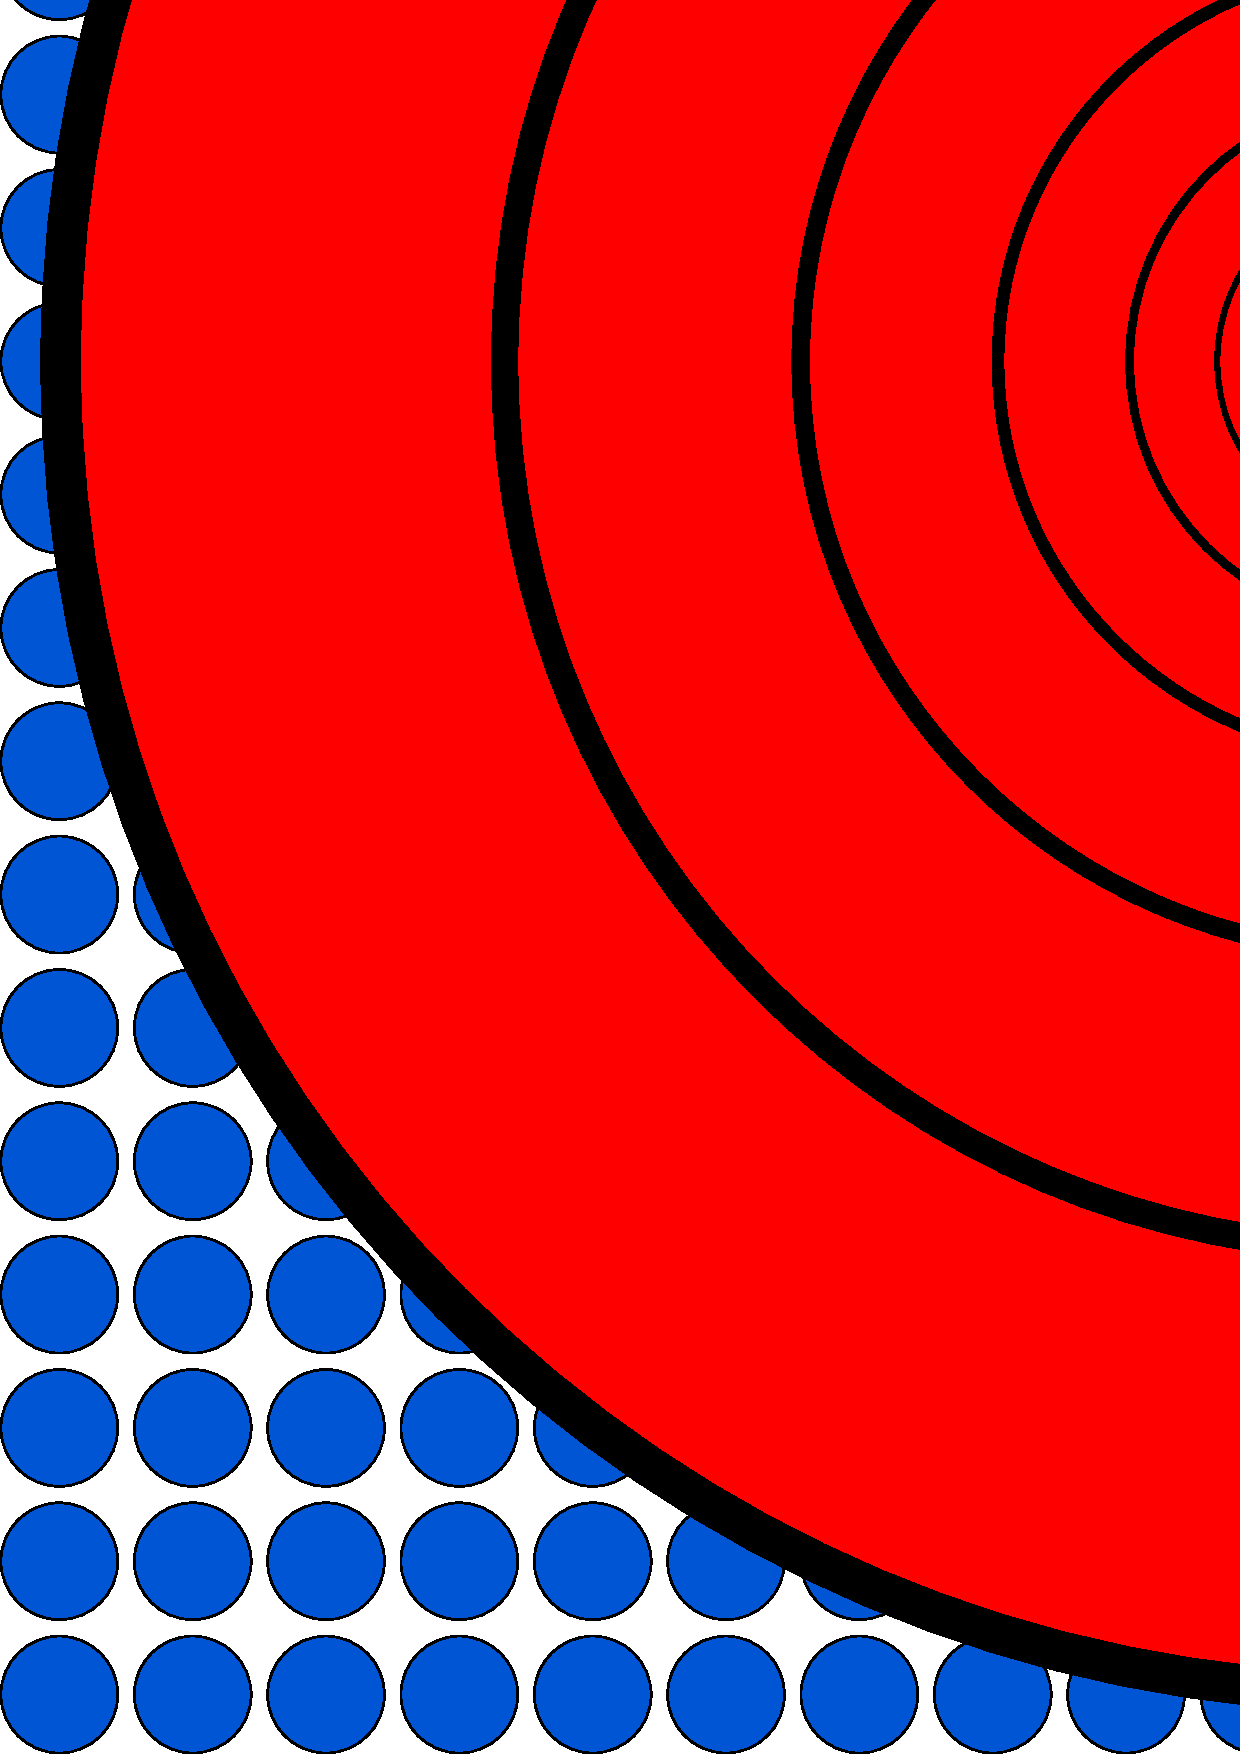
\includegraphics[width=7cm]{fieldsGaussians.png}
\caption{Neural fields for stability control}
\end{figure}


\section{Evolution of Neural Fields}
\subsection{Neural Field Controller Architecture}
The architecture used for the neural field controller uses a structure
similar to that of multilayer perceptrons, i.e. an input layer, a
hidden layer and an output layer. The hidden layer has the properties
so far presented in the neural field model. The input and output layers are also
modelled as a population of neurons but without inner
dynamics. Nonetheless, it is used a kernel for the connection from the
input layer to the hidden layer, as well for the connection from the
hidden layer to the output layer.
The input layer is used as a buffer where sensory inputs are placed
before they are processed by the hidden layer. The output layer is
used so that it can be applied some form of post-processing to the
output of the hidden layer without changing the inner dynamics of the
neural field.

\subsection{Evolutionary Algorithm Structure and Parameters}
For the evolution process it is used a simple evolutionary algorithm
as shown in the preliminaries, with random elimination of individuals
inversely proportional with its fitness.

% , but with the addition of niching in the
% for of Deterministic Crowding (see \cite{referencia-dc}), in order to
% promote additional diversity and to prevent premature convergence.

The evolution parameters are the connection kernels between the input
layer and the hidden layer, and between the hidden layer and the
output layer. The recurrent connections of the hidden layer with
itself are left fixed, in the form of a wizard hat function.

The connection kernels are considered isotropic and homogeneous along
the field, so that they can be described as symmetric one-dimensional
arrays of values. 

\subsection{Genotypic Representation and Evolution Operators}
Each connection kernel can be represented as an array of $N$ values from
$w(0)$ to $w(p)$ with homogeneous spacing, using its symmetry. This
way, for an equal boundary radius for all the kernels, and a 3-layered
architecture, there are $3N$ real values in the genotype. As can be
seen, the number of evolution parameters does not have a direct
relation with the simulation size of the neural fields (the number of
discrete points used), in contradistinction with recurrent neural
networks, where the number of parameters depends on the
number $n$ of neurons with a polynomial order $O(n^2)$.

\subsection{Fitness Functions}
The fitness functions were selected in such a way that the stability controller
only has the goal to reduce inclination, while the positioning
controller has to take into account both inclination and position. The
fitness functions were tuned experimentally to attain a convergence
velocity suitable for the experiment. This has in mind a notion of
sequential evolution of, first, the capability to attain equilibrium,
and later, the capability to perturb the equilibrium controller in
such a way that a planned objective can be reached. 

The fitness function for the stability controller is:

\begin{equation}
F_1(\theta )=100-\frac{100\theta ^4}{\theta _{max}^4 T_{total}}
\end{equation}

And for the positioning controller is:

\begin{equation}
F_1(\theta ,e_x)=100-\frac{100(\theta ^4+e_x^4)}{(\theta _{max}^4+e_{x,max}^4) T_{total}}
\end{equation}


\section{Experimental Framework}
The model used consists of an approach to biped walking based on a
inverted pendulum (car-and-pole) system in which the pendulum equilibrium is looked
for. Nonetheless, supposing that the pendulum mass represents the body
center of mass, it is proposed that is reasonable to expect a system
with its sole function being to stabilize the body. This way, the
navigation system has as purpose to carefully perturb the first controller
in such a way that the stabilizing controller moves the car to the
desired position.

\subsection{Dynamic Model}
The dynamic model used, in mathematical terms, is expressed in the two
equations:

\begin{align}
\ddot{x}&=\frac{F+ml\dot{\theta}^2\sin\theta-mg\cos\theta\sin\theta}{M+m\sin^2\theta}\\
\ddot{\theta}&=\frac{(M+m)g\sin\theta-F\cos\theta-ml\dot{\theta}^2\sin\theta\cos\theta}{l(M+m\sin^2\theta)}+\frac{\tau}{ml^2}
\end{align} 

This model consists of four state variables and a high non-linearity
as it departs from equilibrium points. It is worth noting that the
wanted equilibrium point is in fact unstable.


\section{A RNN Approach for Comparison}
The proposed architecture for the recurrent neural network controller
has two expert recurrent networks, whose interaction will achieve
positioning and equilibrium as well.

There has been applied a preprocessing stage previous to the input
neurons, so that the actual values are not used and instead the inputs
are mapped to 3 fuzzy sets. In this way, the stability controller only
has 3 inputs, while the positioning controller has 6, corresponding to
the same 3 inputs previously described and another 3 due to the fuzzy
mapping of the error signal. All neurons are interconnected and the
first one of them is selected as output without loss of
generality. The neural network topology for the first controller
(stability) is shown in the figure \ref{fig:rnn-arch}.

\begin{figure}[t]
\label{rnn-arch}
\centering
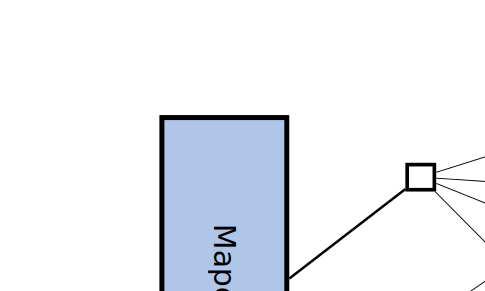
\includegraphics[width=7cm]{rnn.png}
\caption{Neural net for stability control including fuzzy mapping}
\label{rnn}
\end{figure}

\subsection{Evolutionary Algorithm Structure for the RNN Controller}
It is expected, based on the approach of artificial life to
evolutionary robotics (Nolfi y Floreano), that the sequential and
cooperative evolution of elements with biological similarity leads to
an specialization in the process of stabilization and positioning
(despite the antagonistic individual goals of each controller because of the
interest of the positioning controller to maximize also the global
performance).

As said, the two steps are executed sequentially, taking the best
individual of the first step to collaborate with the individual
evolved in the second step. 

Aiming to obtain a fixed length representation and limit the problem
dimensionality, it is used a model of order $Q$ totally connected. Any
network with an order equal or lesser and with total or partial
connections can be represented by the proposed model, by the addition
of activating/deactivating elements for neurons and
connections. Therefore, individual are codified as: 

\begin{itemize}
 \item A bit sequence representing a serialization of an activation matrix
   $A_a$ of dimension $Q$-by-$Q$ which activates/deactivates a
   recurrent connection.
 \item A sequence of real numbers representing a serialization of
   matrices $W_a$ and $W_b$, of dimension $Q$-by-$Q$ and
   $Q$-by-$(m+1)$ respectively.
\end{itemize}

The $C$ matrix is not evolved because it is chosen arbitrarily only
one output (the first neuron). 

The evolution operations used in both steps are:
\begin{itemize}
 \item Parametric mutation of inputs: Gaussian modification of real
   codified matrix weights, which varies connection weights of inputs.
 \item Parametric mutation of recurrences: Gaussian modification of real
   codified matrix weights, which varies connection weights of recurrences.
 \item Selection: Calculates population fitness, selects with elitism
   and culling (5\% of both) couples of parents for generating new
   offsprings, calculates the fitness function for both offsprings.
\end{itemize}

The fitness functions used are the same presented for the neural field controller.

\section{Experimental Set-up}
\label{sec:setup}

The model used consists of an approach to biped walking based on a
inverted pendulum (car-and-pole) system in which the pendulum equilibrium is looked
for. Nonetheless, supposing that the pendulum mass represents the body
center of mass, it is proposed that is reasonable to expect a system
with its sole function being to stabilize the body. This way, the
navigation system has as purpose to carefully perturb the first controller
in such a way that the stabilizing controller moves the car to the
desired position. Here we are particularly interested only on the
stability problem and controller.

\subsection*{Dynamic Model}
The dynamic model used, in mathematical terms, is expressed in the two
equations:

\begin{align}
\ddot{x}&=\frac{F+ml\dot{\theta}^2\sin\theta-mg\cos\theta\sin\theta}{M+m\sin^2\theta}\\
\ddot{\theta}&=\frac{(M+m)g\sin\theta-F\cos\theta-ml\dot{\theta}^2\sin\theta\cos\theta}{l(M+m\sin^2\theta)}+\frac{\tau}{ml^2}
\end{align} 

This model consists of four state variables and a high non-linearity
as it departs from equilibrium points. It is worth noting that the
wanted equilibrium point is in fact unstable.

The output from the stability controller maps to the lateral force
$F$. The angular actuator with value $\tau$ is left to a value of
zero, to allow the plant to behave according to its natural dynamics
on the angular coordinate.


\section{Experimental Results}
\subsection*{Experimentation Details}
The sampling time used was 0.04s (for neural networks, neural fields, and
visualization) and were performed 20s tests.

The differential equation system was solved by a numerical method,
4th Order Runge-Kutta. The iteration step selected was $h=0.002s$ for
each test.

Here are shown the results for the proposed neural field architecture
without evolution and an appropriate selection of parameters (made
taking in account the self-stability of the neural fields and the time
constants of the plant), and the evolution of a recurrent neural
network of a recurrent neural network controller.

\subsection*{Results}
The first experiment tests the physical model using the recurrent
neural network controller without evolution, to see the natural dynamics of the system when the
controller is configured arbitrarily (in such a way that can be perceived
the need of the evolutionary algorithm for the recurrent neural
network controller). Results are shown in the figure
\ref{inestabilidad}. As can be seen, it is an unstable system in the
origin. Red dots represent the pendulum position referenced to
universal coordinates, and blue dots represent the base (car)
position.


\begin{figure}[t]
\centering
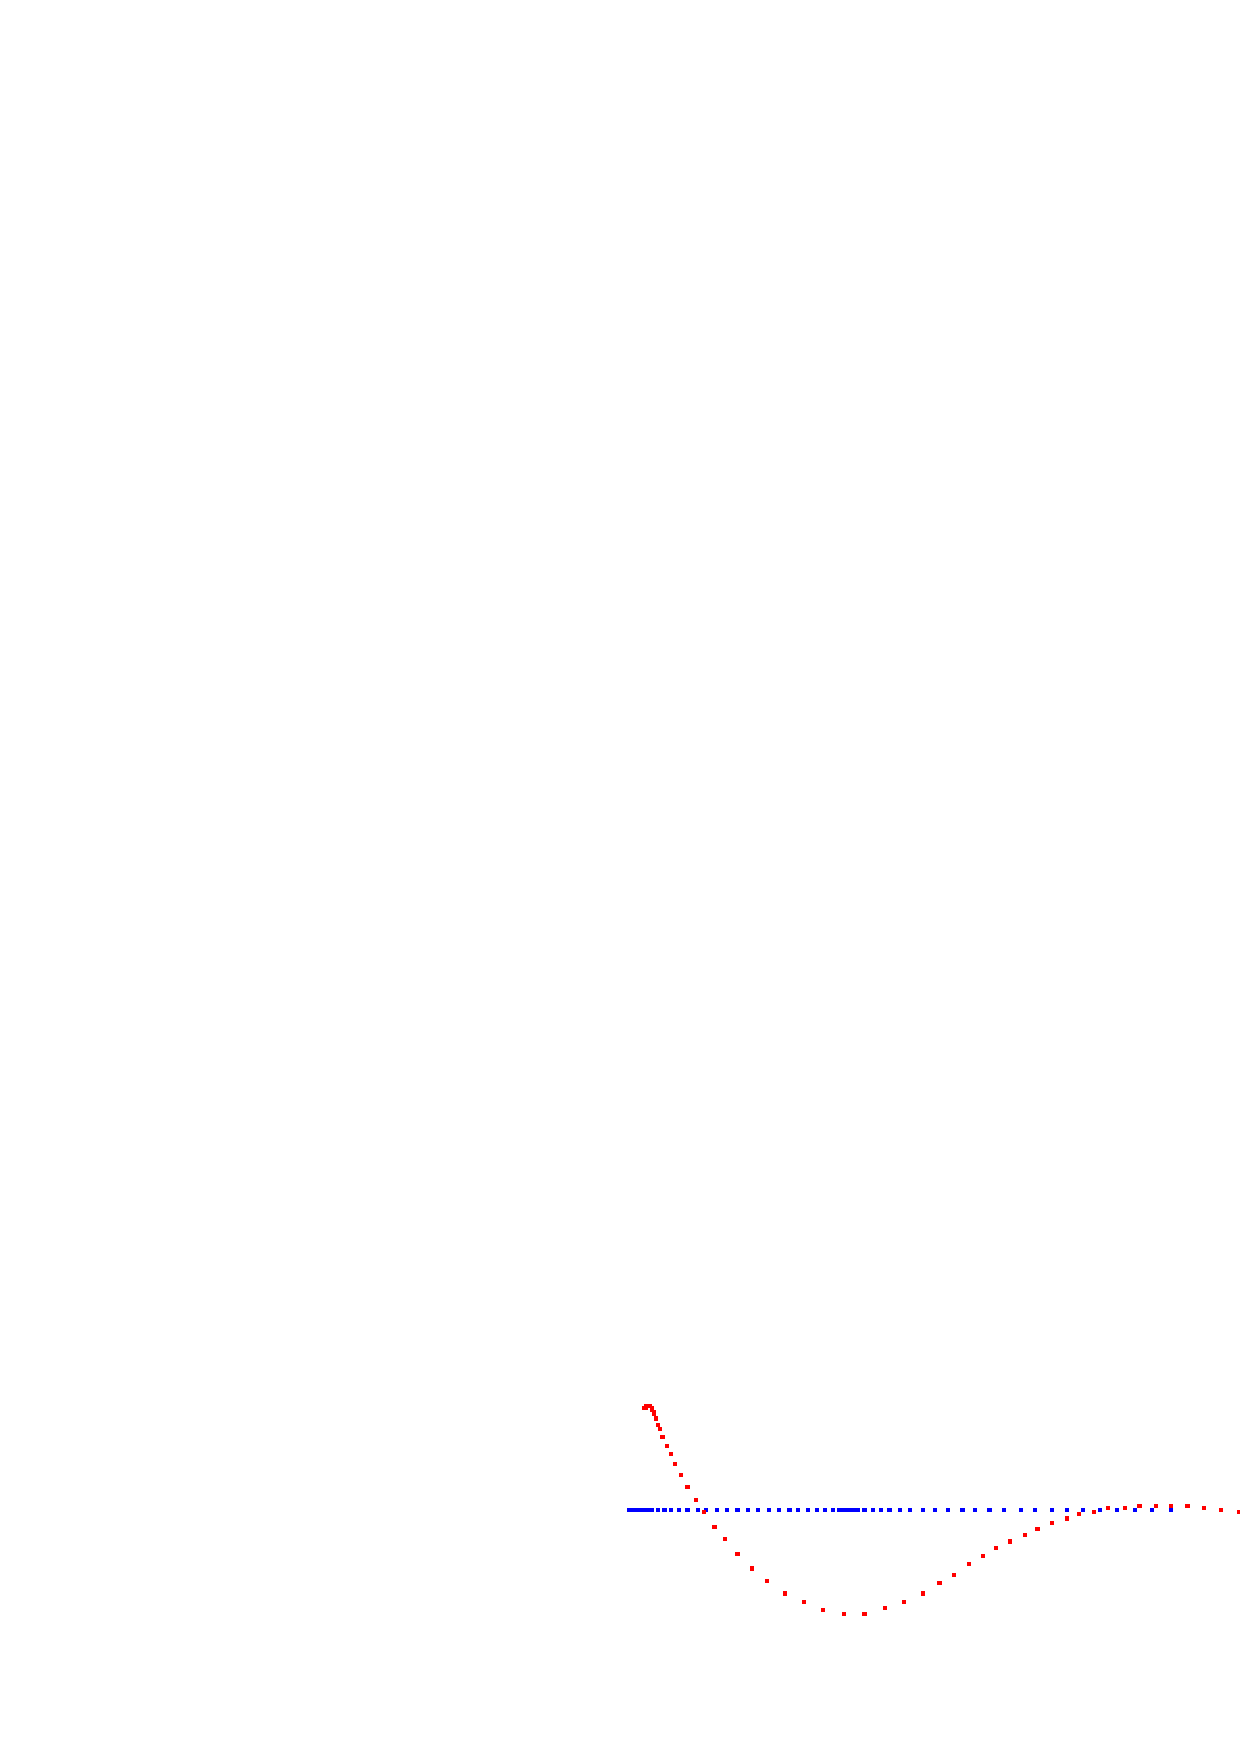
\includegraphics[width=7cm]{inestabilidadG.png}
\\
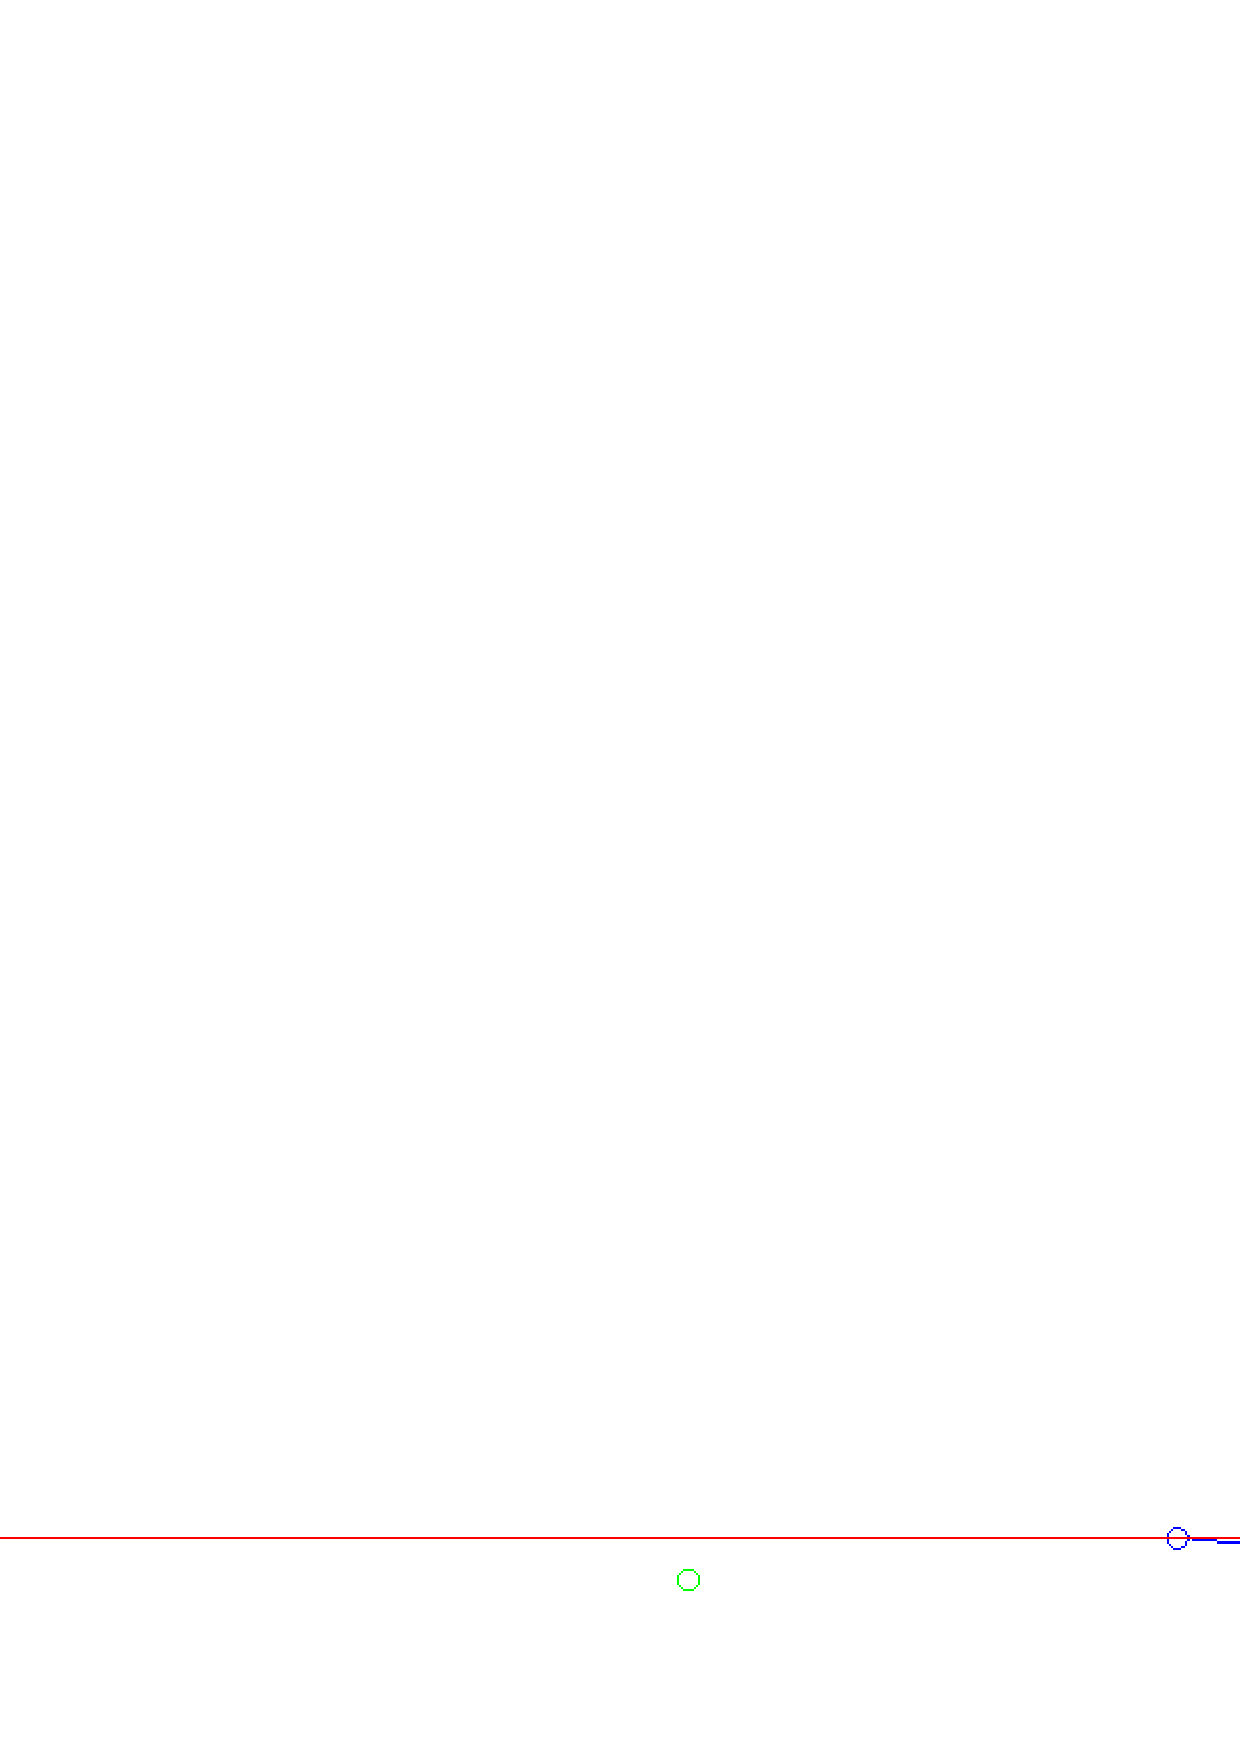
\includegraphics[width=7cm]{inestabilidadC.png}
\caption{System dynamics with an untrained controller}
\label{inestabilidad}
\end{figure}

After the first step of the algorithm, and once done the stability
controller evolution, it is shown the behavior withdrawing the
positioning controller in the figure \ref{final}. The evolution was performed with a population
of 50 individuals and 300 iterations.

\begin{figure}[t]
\centering
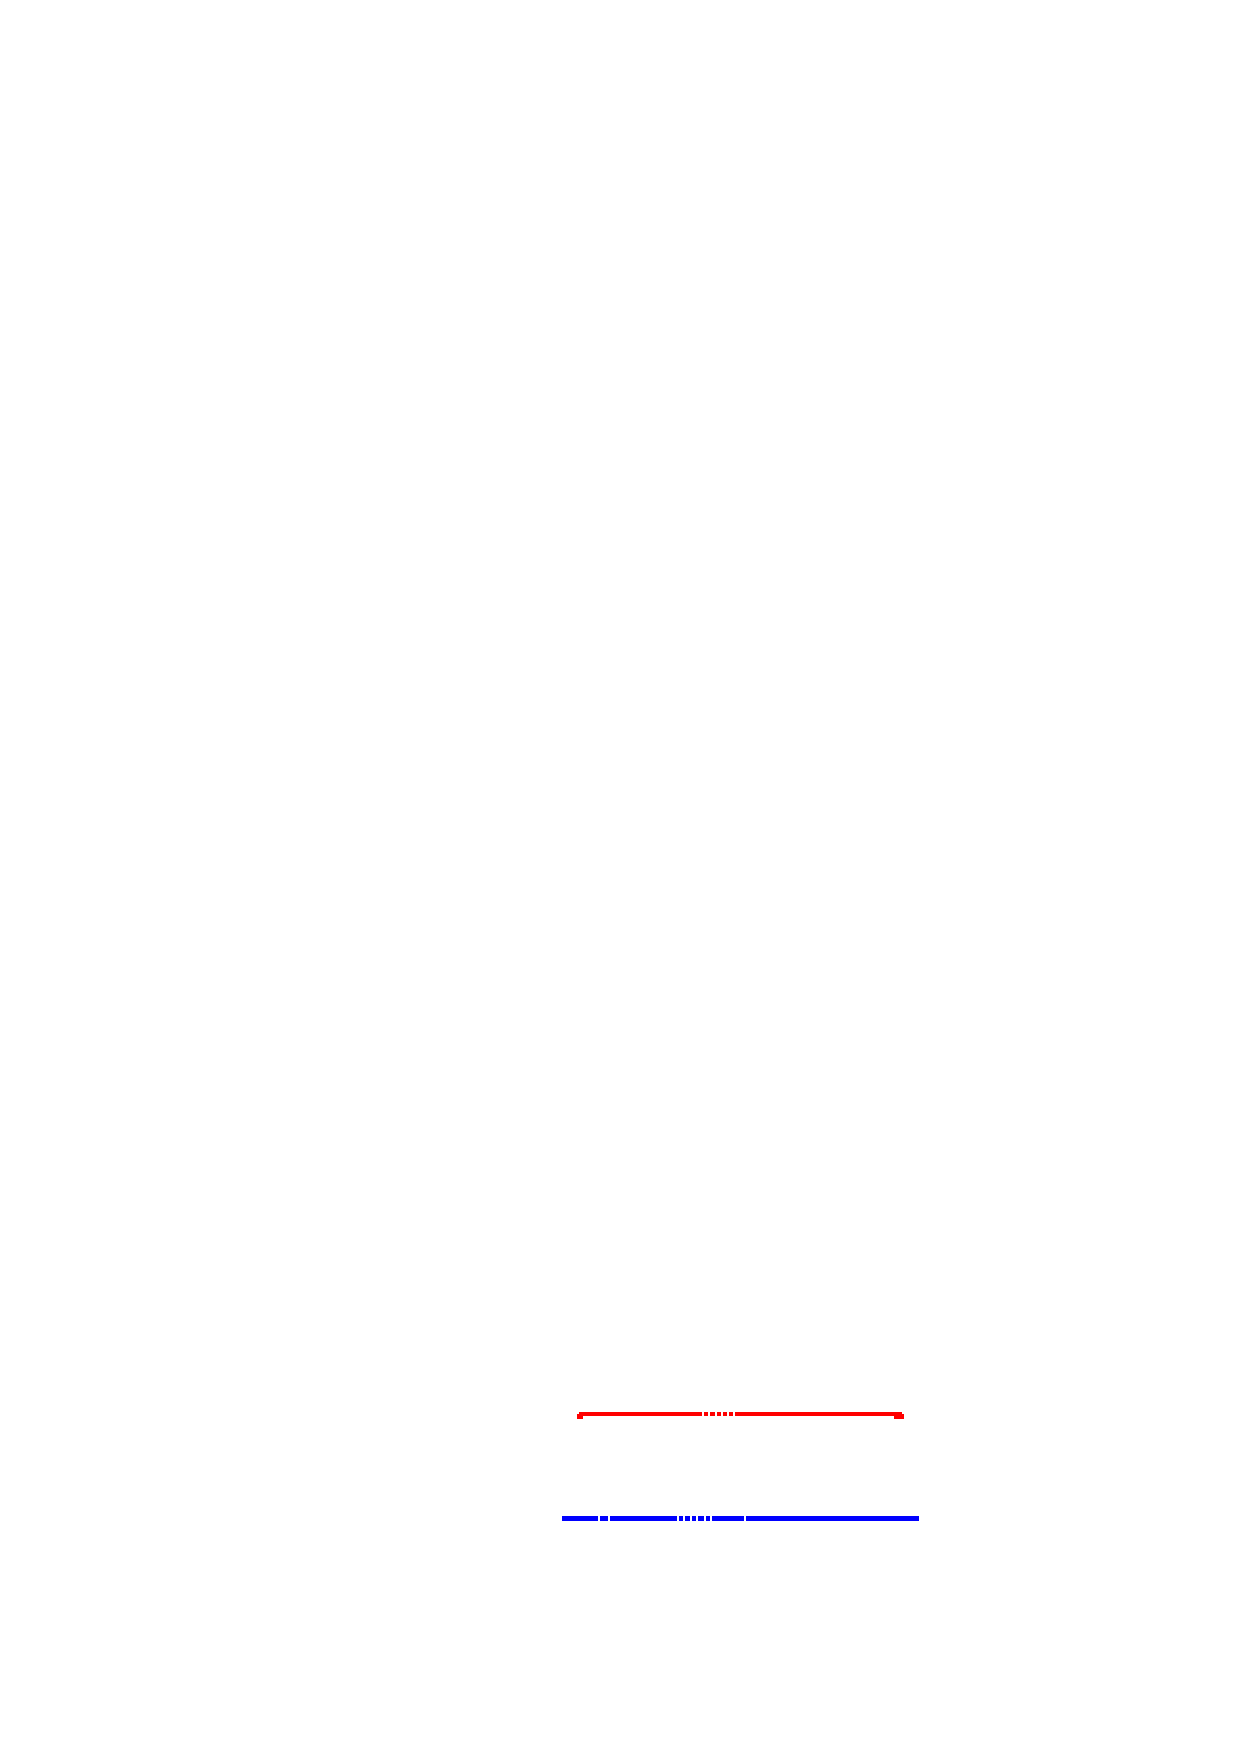
\includegraphics[width=7cm]{finalG.png}
\\
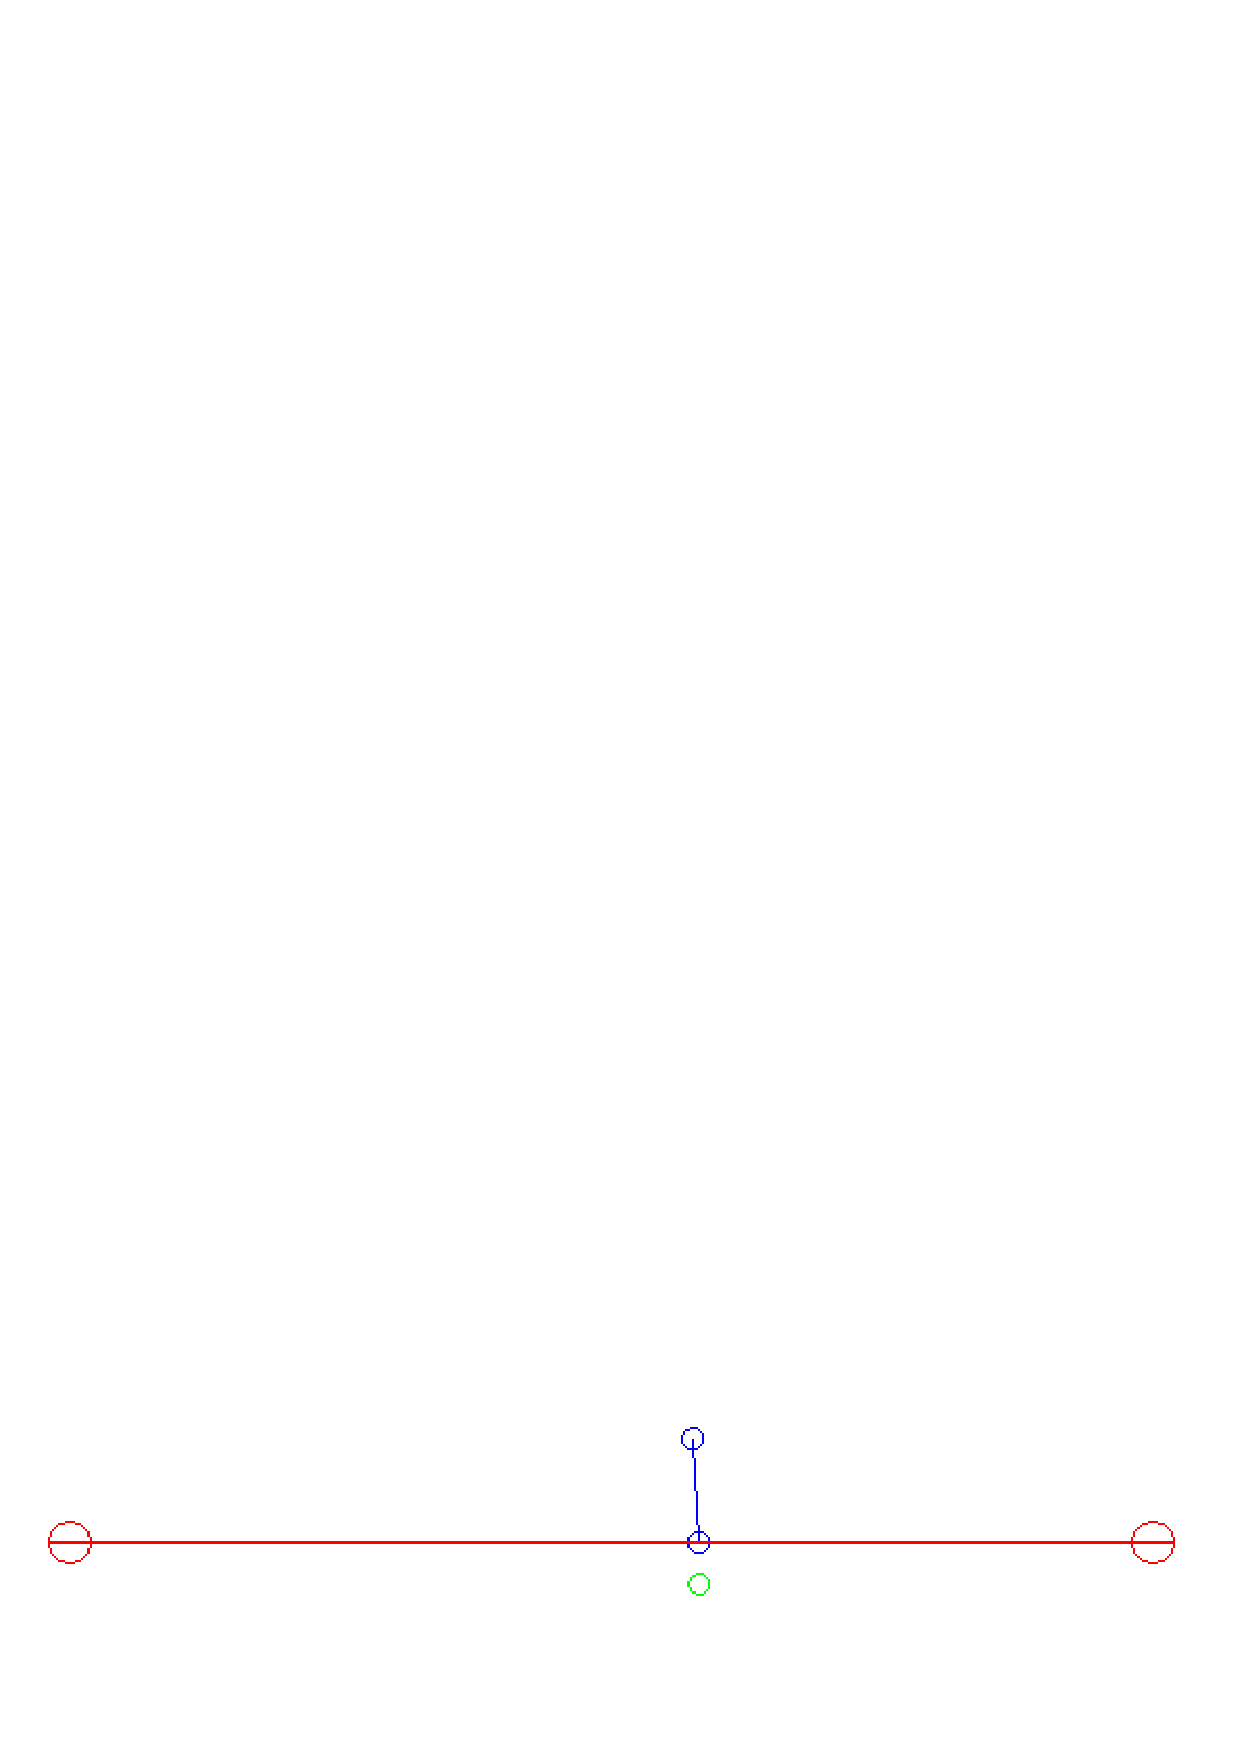
\includegraphics[width=7cm]{finalC.png}
\caption{System dynamics with a RNN controller trained.}
\label{final}
\end{figure}

On the other hand, when the initial angular perturbation is small, the
neural field is able to control the stability without evolution. The
simulation is shown in the figure \ref{estabilidad}.


\begin{figure}[t]
\centering
\includegraphics[width=7cm]{estabilidadG.png}
\\
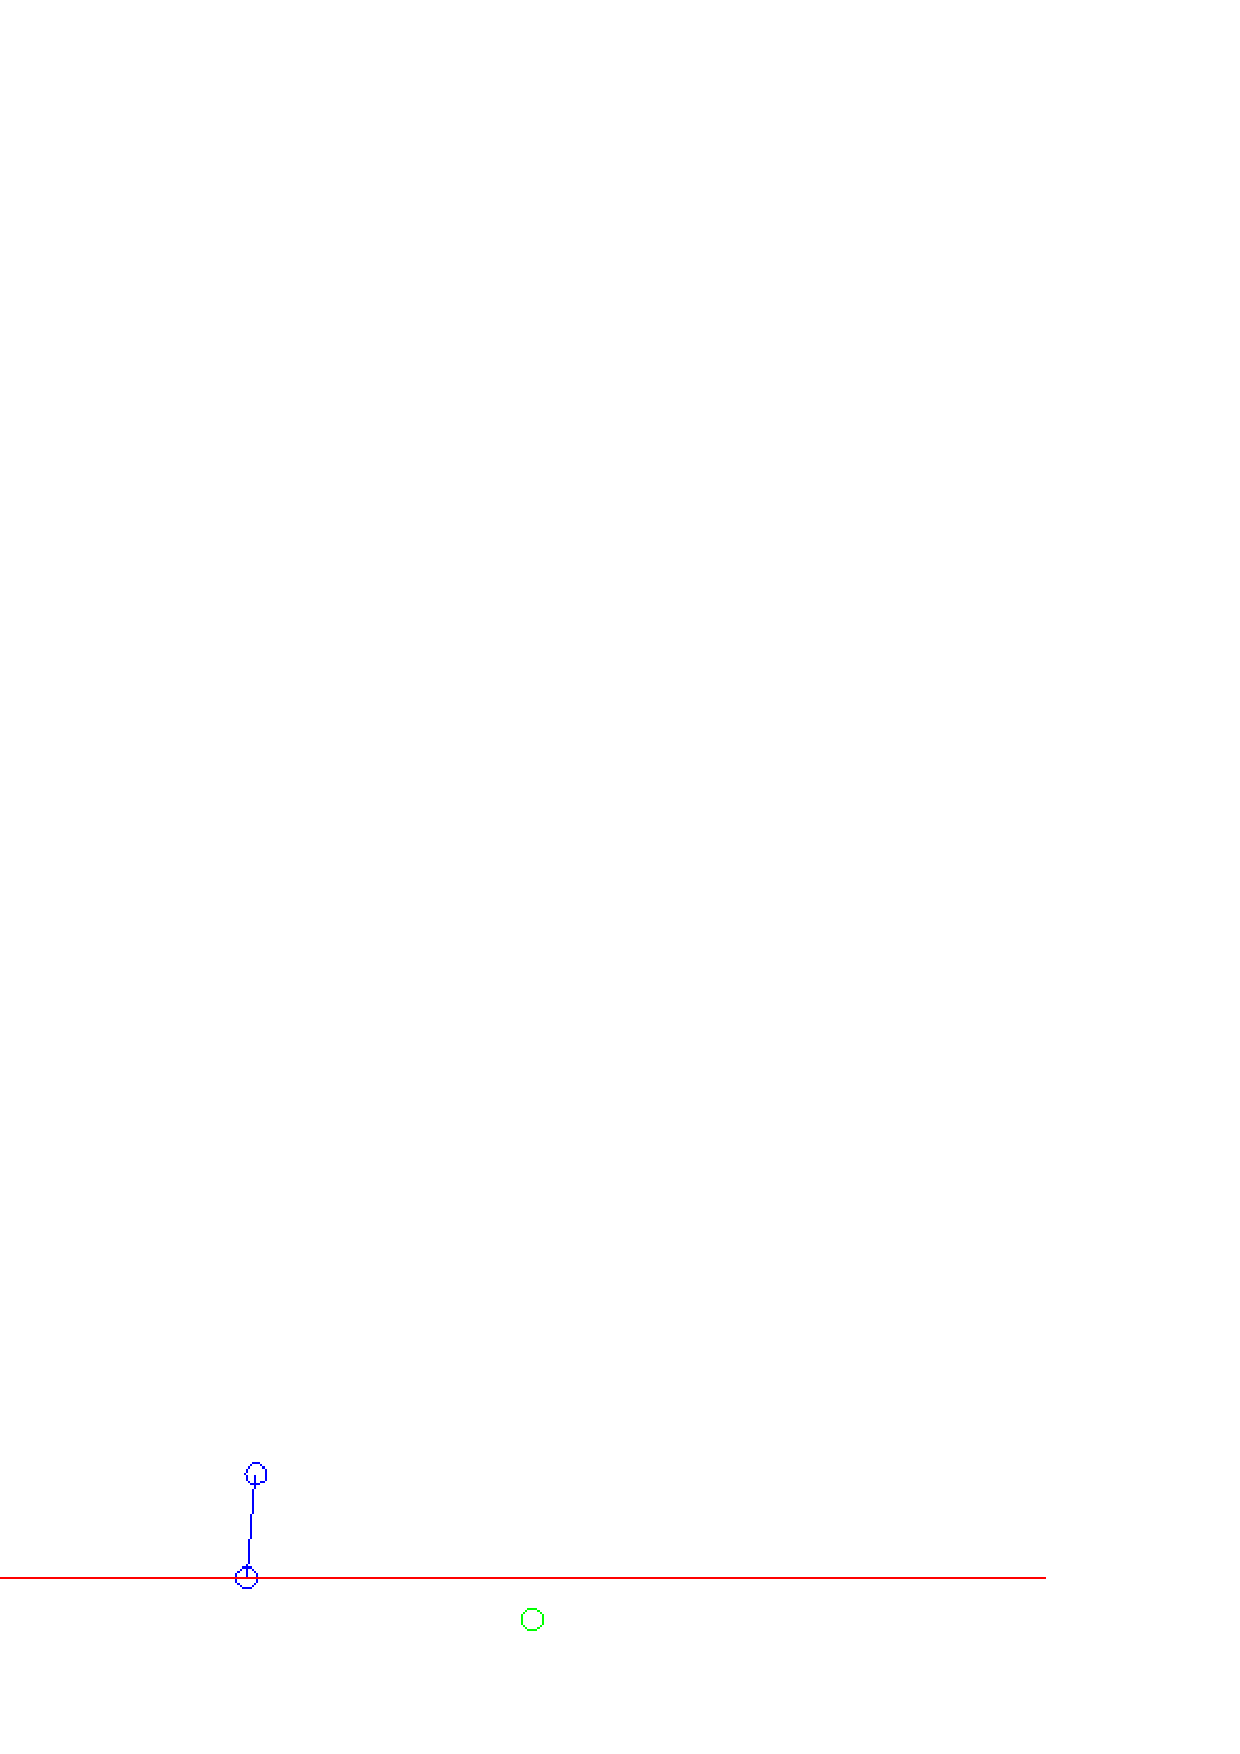
\includegraphics[width=7cm]{estabilidadC.png}
\caption{System dynamics with a non-trained Neural Field Controller.}
\label{estabilidad}
\end{figure}

The output from the processing field can be seen in the figure
\ref{fig:nf-result}.


\begin{figure}[t]
\centering
\includegraphics[width=7cm]{camposC.png}
\caption{Processing Neural Field simulation.}
\label{estabilidad}
\end{figure}



\section{Discussion}
The results obtained from this chapter can be summarized in a short
analysis. 

While the recurrent neural network controller is expressive
enough to solve the problem at hand, the number of parameter to
configure (or in this case to evolve) is of a quadratic order in
relation to the number of nodes (or neurons). This were not a
particular problem for the evolutionary algorithm used, but limits its
potential scalability. Furthermore, while it is expressive enough,
does not show a particular suitability to the dynamic stability
problem of the inverted pendulum and there are no reasons to expect
something different for a more complex biped model. 

On the other hand, the neural field controller is a bit more complex
and its simulation more costly, but has some notable advantages. The
first one is its ability to self-compensate or, equivalently, the
stability of its natural dynamics, which is attained after the setup
of few parameters. The second one is it suitability to the problem at
hand, being able to solve it with a acceptable degree of performance
for small perturbations. Although there was a need to parameter
configuration, evolution was not required because the small number of
parameters to setup: basically three parameters of the kernel function
and the resting potential of the field equation - a number of
parameters of constant order in relation to the number of nodes (point potentials
on the neural field).

It is left for next chapters the challenging but promising task of
neural field evolution.









    %and files

% \input{bibliography}

\end{document}

\message{ !name(thesis.tex) !offset(-62) }
